%%
%% This is file `sample-acmsmall-conf.tex',
%% generated with the docstrip utility.
%%
%% The original source files were:
%%
%% samples.dtx  (with options: `all,proceedings,bibtex,acmsmall-conf')
%% 
%% IMPORTANT NOTICE:
%% 
%% For the copyright see the source file.
%% 
%% Any modified versions of this file must be renamed
%% with new filenames distinct from sample-acmsmall-conf.tex.
%% 
%% For distribution of the original source see the terms
%% for copying and modification in the file samples.dtx.
%% 
%% This generated file may be distributed as long as the
%% original source files, as listed above, are part of the
%% same distribution. (The sources need not necessarily be
%% in the same archive or directory.)
%%
%%
%% Commands for TeXCount
%TC:macro \cite [option:text,text]
%TC:macro \citep [option:text,text]
%TC:macro \citet [option:text,text]
%TC:envir table 0 1
%TC:envir table* 0 1
%TC:envir tabular [ignore] word
%TC:envir displaymath 0 word
%TC:envir math 0 word
%TC:envir comment 0 0
%%
%% The first command in your LaTeX source must be the \documentclass
%% command.
%%
%% For submission and review of your manuscript please change the
%% command to \documentclass[manuscript, screen, review]{acmart}.
%%
%% When submitting camera ready or to TAPS, please change the command
%% to \documentclass[sigconf]{acmart} or whichever template is required
%% for your publication.
%%
%%
\documentclass[acmsmall,screen,review,anonymous]{acmart}
% \documentclass[acmsmall,screen]{acmart}

%%
%% \BibTeX command to typeset BibTeX logo in the docs
\AtBeginDocument{%
  \providecommand\BibTeX{{%
    Bib\TeX}}}

%% Rights management information.  This information is sent to you
%% when you complete the rights form.  These commands have SAMPLE
%% values in them; it is your responsibility as an author to replace
%% the commands and values with those provided to you when you
%% complete the rights form.
\setcopyright{acmlicensed}
\copyrightyear{2018}
\acmYear{2018}
\acmDOI{XXXXXXX.XXXXXXX}
%% These commands are for a PROCEEDINGS abstract or paper.
\acmConference[Conference acronym 'XX]{Make sure to enter the correct
  conference title from your rights confirmation email}{June 03--05,
  2018}{Woodstock, NY}
%%
%%  Uncomment \acmBooktitle if the title of the proceedings is different
%%  from ``Proceedings of ...''!
%%
%%\acmBooktitle{Woodstock '18: ACM Symposium on Neural Gaze Detection,
%%  June 03--05, 2018, Woodstock, NY}
\acmISBN{978-1-4503-XXXX-X/2018/06}


%%
%% Submission ID.
%% Use this when submitting an article to a sponsored event. You'll
%% receive a unique submission ID from the organizers
%% of the event, and this ID should be used as the parameter to this command.
%%\acmSubmissionID{123-A56-BU3}

%%
%% For managing citations, it is recommended to use bibliography
%% files in BibTeX format.
%%
%% You can then either use BibTeX with the ACM-Reference-Format style,
%% or BibLaTeX with the acmnumeric or acmauthoryear sytles, that include
%% support for advanced citation of software artefact from the
%% biblatex-software package, also separately available on CTAN.
%%
%% Look at the sample-*-biblatex.tex files for templates showcasing
%% the biblatex styles.
%%

%%
%% The majority of ACM publications use numbered citations and
%% references.  The command \citestyle{authoryear} switches to the
%% "author year" style.
%%
%% If you are preparing content for an event
%% sponsored by ACM SIGGRAPH, you must use the "author year" style of
%% citations and references.
%% Uncommenting
%% the next command will enable that style.
%%\citestyle{acmauthoryear}


% \usepackage{tcolorbox}
\usepackage{multirow}
\usepackage{longtable}
\usepackage{array} 
\usepackage{booktabs,multirow,array}
\usepackage{graphicx}
\usepackage{caption}
\usepackage{xcolor}
\usepackage{colortbl}
\usepackage{tabularx}
\usepackage{listings}
\usepackage[most]{tcolorbox}

\definecolor{main}{HTML}{5989cf}    % setting main color to be used
\definecolor{sub}{HTML}{cde4ff}     % setting sub color to be used

\newtcolorbox{boxB}{
    enhanced,
    boxrule = 0pt,
    colback = sub,
    borderline west = {1pt}{0pt}{main}, 
    borderline west = {0.75pt}{2pt}{main}, 
    borderline east = {1pt}{0pt}{main}, 
    borderline east = {0.75pt}{2pt}{main}
}


\lstdefinestyle{cotlisting}{
  basicstyle=\ttfamily\scriptsize, % 字体更小：scriptsize（想再大点可改 footnotesize）
  columns=fullflexible,
  keepspaces=true,
  breaklines=true,
  breakatwhitespace=false,
  frame=single,
  framerule=0.4pt,
  rulecolor=\color{black!35},
  xleftmargin=0.6em,
  xrightmargin=0.6em,
  aboveskip=0.6em,
  belowskip=0.2em,
  showstringspaces=false,
  upquote=true,
  backgroundcolor=\color{black!2}
}



%%
%% end of the preamble, start of the body of the document source.
\begin{document}

%%
%% The "title" command has an optional parameter,
%% allowing the author to define a "short title" to be used in page headers.
\title{Fine-grained ML SATD Classification with Large Language Models: An Empirical Study}

% \title{Can Large Language Models Classify Fine-Grained Self-Admitted Technical Debt in Machine Learning Software? An Empirical Study}

%%
%% The "author" command and its associated commands are used to define
%% the authors and their affiliations.
%% Of note is the shared affiliation of the first two authors, and the
%% "authornote" and "authornotemark" commands
%% used to denote shared contribution to the research.
\author{Zhiwei Fei}
\email{zhiweifei@smail.nju.edu.cn}
\author{Yizheng He}
\author{Xing Zhang}
\affiliation{%
  \institution{National Key Laboratory for Novel Software Technology, Nanjing University}
  \city{Nanjing}
  \country{China}}

\author{Zhifei Yang}
\affiliation{%
  \institution{School of Computer Science, Peking University}
  \city{Beijing}
  \country{China}}


\author{Liguo Huang}
\affiliation{%
  \institution{Department of Computer Science, Southern Methodist University}
  \city{University Park}
  \state{Texas}
  \country{USA}}

\author{Jidong Ge}
\authornote{Corresponding Author.}
\affiliation{%
  \institution{National Key Laboratory for Novel Software Technology, Nanjing University}
  \city{Nanjing}
  \country{China}}

%%
%% By default, the full list of authors will be used in the page
%% headers. Often, this list is too long, and will overlap
%% other information printed in the page headers. This command allows
%% the author to define a more concise list
%% of authors' names for this purpose.
\renewcommand{\shortauthors}{Zhiwei Fei et al.}

%%
%% The abstract is a short summary of the work to be presented in the
%% article.
\begin{abstract}
Identifying self-admitted technical debt (SATD), which developers explicitly document in source-code comments, is an important step toward managing software quality. Although SATD has been widely studied in traditional software systems, machine learning (ML) software introduces additional maintenance concerns that are related to data processing, model configuration, dependencies, reliability, and prediction quality. These concerns make ML SATD more fine-grained and difficult to classify than traditional SATD. Existing studies have mainly focused on manually constructing taxonomies and qualitatively characterizing ML-specific SATD. However, it remains unclear whether such fine-grained debt categories can be automatically classified in low-resource settings. This paper presents an empirical study of large language models (LLMs) for fine-grained ML-SATD classification. Using a processed version of the OBrien dataset with 23 ML-specific SATD categories, we evaluate nine LLMs under different prompting strategies, including direct label selection, binary decomposition, hierarchical prompting, LLM-generated examples, and reasoning-oriented prompts. Our results show that LLMs provide a promising solution for this low-resource classification task. Vanilla and binary prompting consistently outperform hierarchical prompting, suggesting that multi-stage label decomposition may introduce error propagation. A small number of generated examples can improve performance, whereas adding more examples does not necessarily lead to further gains. Reasoning-oriented prompting further improves classification effectiveness. By combining these strategies, the best LLMs Qwen-8B achieve a weighted F1-score of 0.381. Our findings provide practical guidance for applying LLMs to ML-SATD classification and a baseline for this area, reveal remaining challenges caused by label imbalance, semantic overlap, and rare debt categories.




\end{abstract}

%%
%% The code below is generated by the tool at http://dl.acm.org/ccs.cfm.
%% Please copy and paste the code instead of the example below.
%%
\begin{CCSXML}
<ccs2012>
   <concept>
       <concept_id>10011007.10011074.10011111.10011696</concept_id>
       <concept_desc>Software and its engineering~Maintaining software</concept_desc>
       <concept_significance>500</concept_significance>
       </concept>
 </ccs2012>
\end{CCSXML}

\ccsdesc[500]{Software and its engineering~Maintaining software}

%%
%% Keywords. The author(s) should pick words that accurately describe
%% the work being presented. Separate the keywords with commas.
\keywords{Self-Admitted Technical Debt, Large Language Models, Low-Resource Text Classification}
%% A "teaser" image appears between the author and affiliation
%% information and the body of the document, and typically spans the
%% page.

% \received{20 February 2007}
% \received[revised]{12 March 2009}
% \received[accepted]{5 June 2009}

%%
%% This command processes the author and affiliation and title
%% information and builds the first part of the formatted document.
\maketitle

\section{Introduction}

% This section is generated by AI
% Machine learning (ML) software has taken an essential role of modern software systems, but its maintenance and evolution remain challenging. Unlike traditional software, whose behaviour is mainly determined by source code, ML software also depends on data pipelines, model configurations, training procedures, external dependencies, and deployment environments. These additional artifacts make maintenance decisions more difficult, because a small change in data preprocessing, model parameters, or library versions may affect prediction quality, reliability, and downstream system behaviour. As a result, technical debt management is particularly important in ML software, where maintainability problems may arise not only from implementation shortcuts, but also from data, model, and pipeline-related decisions.

In recent years, the rapid advances and widespread adoption of artificial intelligence (AI), especially machine learning (ML) and deep learning (DL), have enabled software systems to address problems that were previously difficult or even infeasible with traditional techniques. ML-enabled systems have been increasingly deployed in various domains, including medical diagnosis~\cite{}, financial fraud detection~\cite{}, autonomous driving~\cite{}, and software engineering~\cite{amershi2019software}. However, while ML components provide powerful capabilities, their fast integration into long-lived software systems also introduces substantial maintenance challenges~\cite{sklavenitis2024measuring}. 


Self-admitted technical debt (SATD) provides a practical way to observe such maintenance concerns. SATD refers to debt that developers explicitly document in source-code comments, such as temporary workarounds, incomplete implementations, fragile assumptions, or code that should be improved in the future~\cite{}. This types of technical debt is also commonly appears in machine learning (ML) software. Figure~\ref{fig:motivation_example} shows an example of ML-specific SATD from the open-source GitHub project \texttt{magpie}. In this example, the developer notes that the current output vector is overly sparse and suggests improving its memory efficiency in a future version. Such comments reflect not only acknowledged design or implementation concerns, but also potential risks that may affect the maintainability and evolution of ML systems. Therefore, identifying the fine-grained types of ML-SATD comments can help developers better understand project risks and support more effective technical debt management.


% Because these comments are written by developers during software development and evolution, they provide direct evidence of developers' awareness of suboptimal decisions. Identifying and classifying SATD is therefore an important step toward technical debt management, as it can help maintainers locate potential quality risks, understand the nature of the debt, and decide whether further inspection or repayment is needed.




% Self-admitted technical debt (SATD) provides a practical way to observe such maintenance concerns. SATD refers to debt that developers explicitly document in source-code comments, such as temporary workarounds, incomplete implementations, fragile assumptions, or code that should be improved in the future. Because these comments are written by developers during software development and evolution, they provide direct evidence of developers' awareness of suboptimal decisions. Identifying and classifying SATD is therefore an important step toward technical debt management, as it can help maintainers locate potential quality risks, understand the nature of the debt, and decide whether further inspection or repayment is needed.



% Although SATD has been extensively studied in traditional software systems~\cite{}, studies on ML SATD still need to be explored.

In recent years, the rapid advances and widespread adoption of artificial intelligence (AI), especially machine learning (ML) and deep learning (DL), have enabled software systems to address problems that were previously difficult or even infeasible with traditional techniques. ML-enabled systems have been increasingly deployed in various domains, including medical diagnosis~\cite{}, financial fraud detection~\cite{}, autonomous driving~\cite{}, and software engineering~\cite{amershi2019software}. However, while ML components provide powerful capabilities, their fast integration into long-lived software systems also introduces substantial maintenance challenges~\cite{sklavenitis2024measuring}. 


Self-admitted technical debt (SATD) provides a practical way to observe such maintenance concerns. SATD refers to debt that developers explicitly document in source-code comments, such as temporary workarounds, incomplete implementations, fragile assumptions, or code that should be improved in the future~\cite{}. This types of technical debt is also commonly appears in machine learning (ML) software. Figure~\ref{fig:motivation_example} shows an example of ML-specific SATD from the open-source GitHub project \texttt{magpie}. In this example, the developer notes that the current output vector is overly sparse and suggests improving its memory efficiency in a future version. Such comments reflect not only acknowledged design or implementation concerns, but also potential risks that may affect the maintainability and evolution of ML systems. Therefore, identifying the fine-grained types of ML-SATD comments can help developers better understand project risks and support more effective technical debt management.



ML SATD is more complex than the traditional SATD. 

~\cite{bhatia2023empirical} ~\cite{} ~\cite{}


These technical debt contain all the traditional SATD and the ML-Specifical SATD~\cite{}. ML software is more complex than traditional software due to that the software including AI components 

Prior work has shown that ML-specific debt is often related to data processing, model configuration, dependencies, model interpretability, prediction quality, and reliability. To better characterize these issues, O'Brien et al. proposed a fine-grained taxonomy of SATD in ML software, covering 23 ML-specific debt categories. These categories capture maintenance concerns that are difficult to represent using conventional SATD taxonomies, such as machine learning knowledge, data processing configuration, model code reusability, prediction quality, and machine learning reliability.


Technical debt is a Existing studies have provided valuable taxonomies and empirical characterizations of ML-specific SATD, but they remain largely manual and descriptive. This limits their practical use in large and evolving ML repositories, where developers may produce many comments and where manually assigning fine-grained debt labels is time-consuming. More importantly, fine-grained ML-SATD classification is more challenging than conventional SATD detection. The task requires distinguishing among many semantically related debt categories, while the available labeled data are limited and highly imbalanced. These characteristics make it difficult to directly apply traditional supervised classifiers, which usually require sufficient labeled examples for each category.

Large language models (LLMs) offer a potential alternative for this low-resource classification setting. Since LLMs can follow natural-language instructions and perform classification through prompting, they may reduce the need for task-specific model training. However, it remains unclear whether LLMs can reliably classify fine-grained ML-SATD comments, and how well are they performanced. The difficulty lies not only in selecting the correct label from a large label set, but also in understanding subtle maintenance concerns expressed in short and informal developer comments. In addition, prompt design may substantially affect classification outcomes. A direct prompt may be simple but cognitively demanding; a hierarchical prompt may reduce the decision space but introduce error propagation; in-context examples may clarify label boundaries but may also add noise; and reasoning-oriented prompts may help models distinguish overlapping categories. To the best of our knowledge, there is no work focus on inversigate these aspect, These motivates our to conducted a systematic empirical investigation.

In this paper, we study how to using LLMs for fine-grained ML-SATD classification. LLMs can effectively classifying fine-grained ML-SATD without the need for task-specifical training. We first select a well constructed and wildly used dataset, \citet{obrien202223} constructed a Using a processed single-label subset of O'Brien et al.'s ML-SATD dataset, we evaluate nine LLMs across multiple prompting strategies. Specifically, we examine direct label selection, binary decomposition, hierarchical prompting, LLM-generated in-context examples, reasoning-guided prompting, and combinations of these strategies. Our goal is not only to measure the performance of LLMs on this task, but also to understand how prompt structure, examples, and reasoning affect their ability to distinguish ML-specific technical debt categories.

We address the following research questions:

\begin{itemize}
    \item \textbf{RQ1:} How do different prompt structures affect LLM-based fine-grained ML-SATD classification?
    \item \textbf{RQ2:} To what extent do generated in-context examples help LLMs distinguish fine-grained ML-SATD categories?
    \item \textbf{RQ3:} How does reasoning guidance influence LLM performance on semantically overlapping ML-SATD labels?
    \item \textbf{RQ4:} Can the effective prompting strategies be combined to further improve LLM-based fine-grained ML-SATD classification?
\end{itemize}






% contemporary software systems
Contemporary software systems have enpowered by AI conpornent, it enpowered lots of softwares and maintaining such systems become cretical. Although development these software are very quickly, maintaining these software remains challenging~\cite{sculley2015hidden}. 


% ML systems depends on lots of piplinesUnlike traditional software, ML systems depend not only on source code but also on data pipelines, model configurations, training procedures, dependencies, and deployment environments. These additional artifacts introduce distinctive maintenance risks and make technical debt management particularly important in ML software. 


% In recent years, the rapid advances and widespread adoption of artificial intelligence (AI), especially machine learning (ML) and deep learning (DL), have enabled software systems to address problems that were previously difficult or even infeasible with traditional techniques. ML-enabled systems have been increasingly deployed in various domains, including medical diagnosis~\cite{}, financial fraud detection~\cite{}, autonomous driving~\cite{}, and software engineering~\cite{amershi2019software}. However, while ML components provide powerful capabilities, their fast integration into long-lived software systems also introduces substantial maintenance challenges. 


% \cite{sklavenitis2024measuring}

% Self-admitted technical debt (SATD) provides a practical way to observe such maintenance concerns. SATD refers to debt that developers explicitly document in source-code comments, such as temporary workarounds, incomplete implementations, fragile assumptions, or code that should be improved in the future. Because these comments are written by developers during software development and evolution, they provide direct evidence of developers' awareness of suboptimal decisions. Identifying and classifying SATD is therefore an important step toward technical debt management, as it can help maintainers locate potential quality risks, understand the nature of the debt, and decide whether further inspection or repayment is needed.









% Developing this software is really cheap and faster, ~\cite{sculley2015hidden} 

% Technical debt was coined by \citet{cunningham1992wycash} to describe situations in which developers need to meet urgent deadlines or address immediate resource constraints and therefore adopt less-than-ideal software design or coding practices. Although this approach may speed up the development process in the short term, such code may be more costly to maintain and may hinder subsequent software evolution.

% Technical debt in AI-system refers to the 



To trace and manage technical debt, prior research has largely focused on self-admitted technical debt (SATD)~\cite{potdar2014exploratory}, a type of technical debt documented by developers in source code comments. Although SATD has been widely studied in traditional software systems, it also commonly appears in machine learning (ML) software. Figure~\ref{fig:motivation_example} shows an example of ML-specific SATD from the open-source GitHub project \texttt{magpie}. In this example, the developer notes that the current output vector is overly sparse and suggests improving its memory efficiency in a future version. Such comments reflect not only acknowledged design or implementation concerns, but also potential risks that may affect the maintainability and evolution of ML systems. Therefore, identifying the fine-grained types of ML-SATD comments can help developers better understand project risks and support more effective technical debt management.



These studies regard the identification and classification of SATD as the first step toward its effective management. Most of them rely on learning-based methods to detect and classify SATD in traditional software systems. In general, these approaches can be summarized in two main steps: 1) collecting a large training dataset, and 2) training a task-specific classifier on the dataset, which is then used to identify and classify SATD~\cite{wattanakriengkrai2019automatic, chen2021multiclass}.


However, when it comes to Self-admitted technical debt in machine learning (ML SATD) these approaches are failed.  ML systems face all the maintenance problems of conventional code, plus an additional set of ML-specific issues. Making it more complex than the SATD taxonomy in traditional software~\cite{recupito2024technical}. There are two main obstracal using learning-based approach to classifiy fine-grained ML SATD. The first one is 1) The label of fine-grained ML SATD is more complex and spare. It involves specialized and more complex types than traditional SATD~\cite{recupito2024technical}. 2) The datasets are really small. It is hard to collect a lots of training datasets which always exceed the testing datasets size and fine-tuning a task specifical model for classification it. As a results, to the best of our knowledge, no work present an automatic method to classify ML SATD. Prior work has proposed taxonomies of SATD in AI-powered systems~\cite{breck2017ml, pepe2024taxonomy} and conducted empirical analyses~\cite{alahdab2019empirical, bhatia2023empirical} of the patterns of these SATD. These studies mainly focus on manually analyzing SATD types in AI-powered systems, they manually the detailed types and patterns can help identify ML SATD and facilitate reducing the maintenance cost of the software. 


% However to the best of our knowledge, previous work didn't present an automatic method to classify the different types of ML SATD. We think fine-grained ML SATD classification encounters two major barriers: 1) lacking sufficient training datasets. 2) The taxonomy of ML SATD types is much more complex than general SATD Types. The lack of sufficient training datasets makes the learning-based methods used in previous work unsuitable for this task. Fine-grained ML SATD types usually involve more labels, and the complex label taxonomy makes the problem more challenging than traditional SATD classification. More recently, some studies have examined the effectiveness of LLMs for SATD identification and classification~\cite{sheikhaei2024empirical, fontana5209087binary}.




% This debt may be difficult to detect because it exists at the system level rather than the code level. Traditional abstractions and boundaries may be subtly corrupted or invalidated by the fact that data influences ML system behavior. Typical methods for paying down code level technical debt are not sufficient to address ML-specific technical debt at the system level.

\begin{figure}[t]
    \centering
    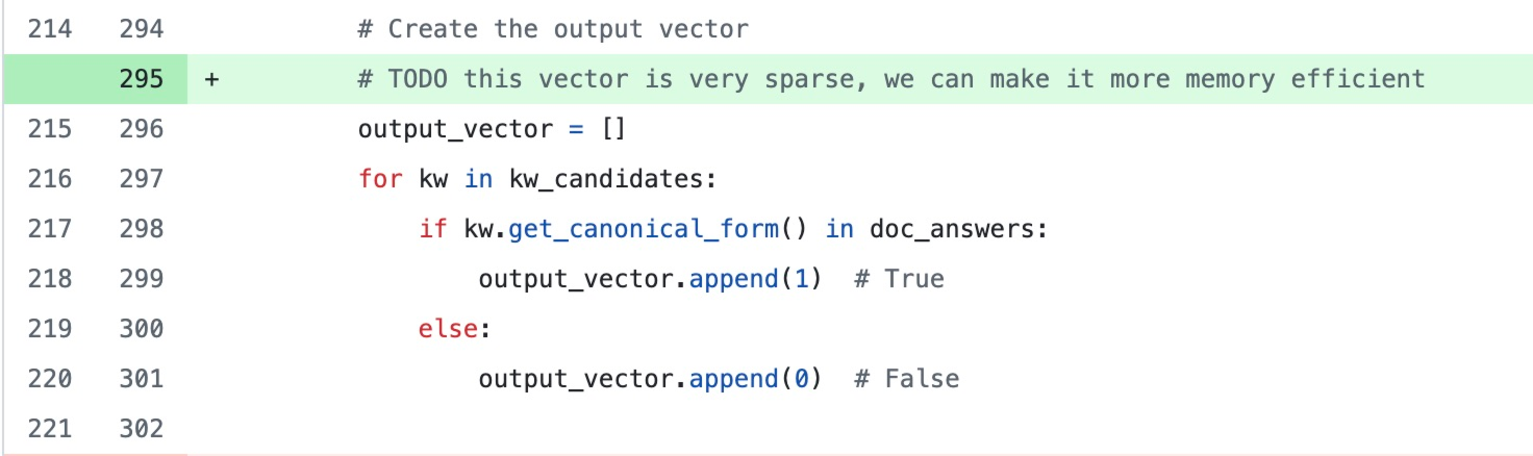
\includegraphics[width=0.8\textwidth]{example_of_ML_SATD.pdf}
    \caption{Example of ML SATD in the open source project.}
    \label{fig:motivation_example}
\end{figure}



Large Language Models (LLMs) have the potential on tackling this problem by using prompting without task-specific training. This method sheild light on the fine-grained ML SATD classification, Some research have study using it to identificy the SATD in traditional software~\cite{}. However their effectiveness on the fine-grained ML SATD classification task still need explored. We fill this gap in this study, we explored how to better using these LLMs on this task. Prompting is the most important thing in this we evaluate different prompting methods. To understanding how to better prompting these LLMs and know their performance on this task. We first explored three prompting methods, 


By addressing these research questions, this study not only sheds light on the current capabilities and limitations of LLMs in the area of ML SATD classification but also provides actionable guidance for leveraging LLMs effectively in software engineering research and practice.


Our empirical study address four research questions:



\textbf{RQ1:} How to prompt LLMs for fine-grained ML SATD classification?

% Prompts are key factors influencing LLMs performance on ML SATD classification. In this RQ, we explore how to design prompts to enhance classification accuracy. We evaluate three prompting strategies vanilla prompt, binary prompting,g and hierarchical prompts. Through these strategies, we aim to provide insights into designing prompts that guide LLMs toward more accurate ML SATD classification.

\textbf{RQ2:} Can incorporating LLM-generated examples improve the performance of LLMs on fine-grained ML SATD classification?

% Many studies suggest that incorporating examples into prompts (few-shot prompting) improves model performance. However, limited dataset sizes make it difficult to provide sufficient examples. In this research question, we investigate whether LLM-generated examples can enhance model performance and how the number of provided examples affects it.


\textbf{RQ3:} Can reasoning improve the performance of LLMs on fine-grained ML SATD classification?

% Requiring LLMs to perform reasoning before answering is becoming increasingly common, as models that generate responses through deeper reasoning often achieve better performance. In this RQ, we aim to evaluate the results of thinking LLMs under the thinking mode and compare them with the non-thinking mode to figure out their influence on the final results. We also test whether manually written Chain-of-Thought can further improve performance, and compare these thinking LLMs with general LLMs.

% non-thinking model with the maually written Chain-of-thought to imitate the thinking process. And 

% using the imitate reasoning prompting, which instructs the model to think step by step and output the reasoning first, followed by the answer, which is conceptually similar to the reasoning mode.

% This RQ will detail the different model settings, including CoT, the thinking mode of models.  




\textbf{RQ4:} Can combining these approaches further improve LLM performance in the fine-grained classification of ML SATD?

% In this RQ, we further explore we will analyze each model's performance from different aspect and compare their performance under different settings and figure out the best practice of using these models. We set two baselines: random guess and the majority class, which selects the most common label as the predictions. This analysis provides insights into how LLMs perform on fine-grained classification of ML SATD.





% With the growing development of LLMs, which can be used through instructions and doesn't need training a specific model for each dataset, sheild light on automated classification of these ML SATD. In this paper, we detailed analysis the way to using LLMs for ML SATD classification. We focus on three aspect, the first one is how to prompt these LLMs to achieve better results. As prompting is the most important things to guide the LLMs to finished the task and we detailed explored three prompting methods, which are vanilla, binary and hierarchical prompting. Incorperating examples into the prompting can improve the performance, however due to lack of sufficient datasets, selecting examples from the datasets is not possible. So we explored whether LLMs generated examples can improve the overall results. The LLMs are turning into reasoning mode which shows impressive performance on the complex tasks. We detailed whether this mode although improve the performance of ML SATD classification. We manually written a Chain-of-thought which contains some guildline to show how to classify the ML SATD, to guiled the classifiaction of the final labels. Finally, we test whether combaination of these methods can further improve the final performance.

\textbf{Summary of findings} We evaluate nine LLMs to reveal how to , and the results show that vanilla and binary prompting are the two most effective prompting strategies for this task (RQ1). We also find that model-generated examples can improve performance, although adding more examples does not necessarily lead to better results; in particular, using no more than three examples yields the best performance (RQ2). In addition, reasoning mode further improves the results, and incorporating manually written chain-of-thought examples helps the models perform better on the classification task (RQ3). By combining these strategies, the best-performing model is Qwen3-8B under the 3-shot setting, achieving an F1 score of 38.1\% (RQ4).



% In particular, fine-grained DL SATD classification faces two practical barriers. First, the DL-specific taxonomy contains many more labels than conventional SATD schemes, increasing ambiguity and exacerbating class imbalance. Second, labeled data at this granularity is expensive to obtain and therefore limited, making it difficult to train robust supervised models without substantial annotation effort. Motivated by the rapid progress of instruction-following LLMs, this paper investigates whether LLMs can serve as a practical alternative for fine-grained DL SATD classification via prompting and label descriptions, reducing reliance on large task-specific training datasets. We systematically evaluate LLM-based classifiers against strong supervised baselines under limited data, and analyze how prompt design and code context influence performance across DL SATD types.





% \cite{bhatia2023empirical}

% \cite{kojima2022large}


Our contributions are fourfold:

(1) We conduct the first and largest empirical study on the performance of LLMs in fine-grained ML SATD classification. A total of nine LLMs, covering both general-purpose and code-oriented models, reasoning models, are evaluated to assess their effectiveness on this task.

(2) We explore different prompting strategies, including vanilla, binary, and hierarchical prompting. The results provide practical guidelines for selecting effective prompts for fine-grained ML SATD classification.

(3) We explored two different ways automatically generated examples and reasoning mode and demonstrate their effectiveness on this task.

(4) We further explore combinations of these prompting methods and report the best performance achieved by current LLMs on this task, which can serve as a strong baseline for future studies.




The rest of the paper is organized as follows. Section \ref{sec:related_work} introduces the LLMs and summarizes the current state of ML SATD classification. Section \ref{sec:methodology} gives the detailed datasets, models, parameters, and evaluation metrics used in this paper and the detailed methodology for each RQ. Section \ref{sec:results} presents the results of each RQ and summarizes the findings. Section \ref{sec:discussion} give a detailed discuss of the lessons learned from the experiments. Section \ref{sec:threats} give the threats to validity. Section \ref{sec:conclusion} concludes our paper.

% Section \ref{sec:motivation_examples} give an example of ML SATD to deep the understanding of ML SATD. Section \ref{sec:research_questions} details the three research questions we want to analyze.


% \section{Motivation Examples}\label{sec:motivation_examples}

% This section can be merged into the Introduction

% % \begin{figure}[H]
% %     \centering
% %     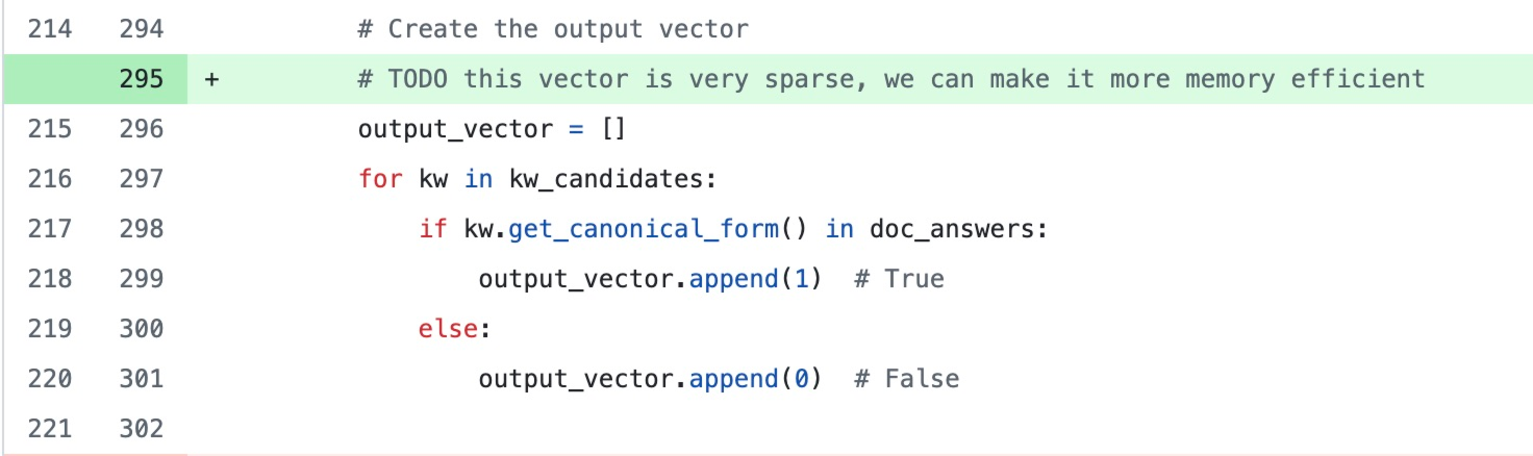
\includegraphics[width=0.8\textwidth]{example_of_ML_SATD.pdf}
% %     \caption{Example of ML SATD in the real life.}
% %     \label{fig:motivation_example}
% % \end{figure}

% Machine learning projects are widely used in our daily lives. The competitive marketing pressure and other deadlines push them to develop quickly and hurry to put their project to the market. Those hush will lead some not optimal solustion be merged into the project. 


% We provide an example in Figure~\ref{fig:motivation_example}, this is a ML SATD which is DS conf type find in the open source github code magpie. The developer find the current output vector is very sparse, and suggest in the next version to make it more memory efficient and this is document in the code comment. Knowing the detailed type of this ML SATD comments will help develper to find the potential project risks and help better manager the project. 


% %按照Empircal Study的格式写。

% Different from traditional technical debt, Classifying ML SATD faces three problems: 1) the first one is SATD is really rare in software projects, so there is not enough training datasets to train a task-specific model to complete this task. Previous work based on the training-based methods can not be applied into this project. 2) Fine-grained ML SATD have more types than traditional SATD. For instance the fine-grained ML SATD have 23 types and with hierarchy information~\cite{}. This make it hard to construct a manually crafted features for different types of labels and can generalized well to different projects.


% LLMs which can solve problems only with instructions shows the protational of automatic classify this ML SATDs and this sherd light for automating this process, but to our best knowledge, no work have excplored this. We give the first large empircal study of the current state of their effectiveness on this task, and give the details on how to instruct this models to get a better performance. 



% \section{Related Work}\label{sec:related_work}
% In this section, we first introduce the LLMs and then describe the current state of ML SATD classification. 
% \subsection{Large Language Models}

% A large language model refers to a model that is pre-trained on massive-scale corpora and often further tuned to follow human instructions more effectively~\cite{zhao2023survey}. LLMs have been 





% \subsection{Self-Admitted Technical Debt Classification}

% Maldonado and Shihab~\cite{maldonado2015detecting} introduced the task of SATD classification. They 


% Classic supervised approaches, including maximum-entropy and other NLP-based pipelines, showed that some SATD categories can be learned across projects, while also revealing the limitations of hand-crafted features and project-specific vocabularies~\cite{da2017using,huang2018identifying,wattanakriengkrai2019automatic}. Later studies moved beyond binary detection to multi-class SATD classification~\cite{chen2021multiclass,ARCELLIFONTANA2025107862}. Structured models such as XGBoost established competitive baselines for canonical SATD categories~\cite{chen2021multiclass}, while deep neural approaches further improved performance by leveraging richer representations and handling class imbalance~\cite{yu2023detecting}. Other work also emphasized interpretability, showing that explanation techniques are useful for understanding model behavior in SATD prediction~\cite{yin2023two}.

% More recently, large language models (LLMs) have opened a new direction for SATD classification~\cite{sheikhaei2024empirical,ARCELLIFONTANA2025107862}. Prior work shows that prompt-based LLMs can achieve competitive results on binary SATD detection and promising, though still uneven, results in multi-class settings~\cite{sheikhaei2024empirical,ARCELLIFONTANA2025107862}. Hybrid methods that combine LLMs with smaller neural models can further improve performance, and recent empirical studies suggest that prompt design materially affects SATD classification outcomes~\cite{li2025large,sheikhaei2024empirical}.

% However, most existing automated SATD research targets traditional software rather than ML-based systems~\cite{chen2021multiclass,da2017using,huang2018identifying,wattanakriengkrai2019automatic,yin2023two,yu2023detecting,sheikhaei2024empirical,ARCELLIFONTANA2025107862}. In contrast, prior work on ML-specific SATD has mainly focused on understanding the nature of debt in ML software instead of automating its fine-grained classification~\cite{obrien202223,bhatia2023empirical,pepe2024taxonomy}. Foundational studies on technical debt in ML argue that ML systems accumulate distinctive forms of debt, such as data and feature dependencies, configuration issues, hidden feedback loops, and pipeline complexity, which are not well captured by generic SATD categories~\cite{sculley2014machine,sculley2015hidden,breck2017ml}. Building on this view, O'Brien et al. proposed a fine-grained taxonomy of SATD in ML software and released a labeled dataset with 23 ML-specialized SATD types~\cite{obrien202223}. More recently, Bhatia et al. provided large-scale empirical evidence that SATD is more prevalent in ML-based systems than in non-ML software, identified data preprocessing and model building as particularly debt-prone stages, and highlighted the need for ML-specific debt management and detection support~\cite{bhatia2023empirical}. These studies also suggest that findings derived from traditional SATD settings or from framework-level analyses cannot be directly transferred to real ML-based systems~\cite{bhatia2023empirical,liu2020using}.

% These studies establish the importance and distinctiveness of ML-specific SATD, but they stop short of providing an automatic solution for fine-grained classification over the ML-specialized taxonomy~\cite{obrien202223,bhatia2023empirical}. This problem is particularly challenging because the available ML-SATD datasets are small and highly imbalanced, while the label space is much more fine-grained than in traditional SATD classification~\cite{obrien202223}. In our setting, the O'Brien dataset contains 23 ML-specialized SATD types, and many categories are sparse~\cite{obrien202223}, which makes training-based approaches difficult to apply reliably. Motivated by the strong in-context learning and reasoning capabilities of LLMs~\cite{liu2023pre,kojima2022large}, our work investigates whether open LLMs can serve as effective classifiers for fine-grained ML-SATD and systematically evaluates prompting, example augmentation, and reasoning strategies for this task.

\section{Related Work}
\label{sec:related_work}

Our work lies at the intersection of two lines of research: automated identification and classification of self-admitted technical debt (SATD), and technical debt in machine learning (ML) software. We review these two areas and position our study with respect to existing SATD classification techniques and ML-specific debt taxonomies.

\subsection{Automated Identification and Classification of Self-Admitted Technical Debt}

SATD refers to technical debt that developers explicitly acknowledge in software artifacts, particularly source-code comments~\cite{potdar2014exploratory}. Early studies investigated the identification and categorization of SATD in traditional software systems~\cite{maldonado2015detecting}. Subsequent work automated SATD detection using natural-language processing, text mining, and supervised learning techniques~\cite{da2017using,huang2018identifying,wattanakriengkrai2019automatic}. Neural models were later introduced to improve representation learning, cross-project prediction, and the interpretability of SATD detection~\cite{ren2019neural}. Collectively, these studies demonstrated that textual information in developer comments can effectively support automated SATD analysis, although most early approaches primarily focused on distinguishing SATD from non-SATD.

Researchers have subsequently extended SATD analysis from binary detection to multi-class classification. \citet{chen2021multiclass} formulated SATD classification as a multi-class learning problem and investigated the use of XGBoost for distinguishing among general SATD categories. Deep-learning approaches have also been explored to improve multi-type SATD classification, particularly under imbalanced class distributions~\cite{yu2023detecting}. More recently, \citet{ARCELLIFONTANA2025107862} systematically revisited binary and multi-class SATD classification, providing an updated assessment of the capabilities and limitations of existing classification techniques. These studies advance automated SATD analysis beyond binary detection, but their classification targets remain predominantly conventional software debt categories.

Large language models (LLMs) have recently provided an alternative to task-specific supervised classifiers. \citet{sheikhaei2024empirical} systematically evaluated LLMs for SATD identification and classification under fine-tuning and in-context learning settings, and examined the effects of demonstrations, category descriptions, model scale, and contextual information. Their results demonstrate the potential of LLMs for SATD analysis and highlight the importance of prompt configuration. However, their classification experiments on the O'Brien dataset consider six general SATD categories---Requirement, Code, Test, Defect, Design, and Documentation---rather than the fine-grained ML-specific taxonomy. Other studies have explored hybrid approaches combining LLMs with smaller neural models~\cite{li2025large}, while \citet{ARCELLIFONTANA2025107862} also evaluated LLMs in multi-class SATD classification. Therefore, although LLM-based SATD classification has received increasing attention, their effectiveness in distinguishing fine-grained ML-specific debt types remains insufficiently understood.

\subsection{Technical Debt and SATD in Machine Learning Software}

ML software introduces maintenance concerns that extend beyond those typically encountered in traditional software. Early studies highlighted forms of technical debt arising from data dependencies, configuration complexity, pipeline entanglement, hidden feedback loops, and interactions among ML components~\cite{sculley2014machine,sculley2015hidden,breck2017ml}. Subsequent empirical studies provided further evidence of domain-specific technical debt in ML and deep-learning systems~\cite{alahdab2019empirical,liu2020using}. More recently, \citet{bhatia2023empirical} investigated SATD in ML software at scale and showed that SATD is prevalent across ML development activities, further motivating dedicated techniques for managing technical debt in ML systems.

To characterize these domain-specific concerns, researchers have developed specialized SATD taxonomies for ML and deep-learning software. \citet{obrien202223} conducted an empirical study of SATD in ML repositories and introduced a fine-grained taxonomy consisting of 23 ML-specific SATD types. These categories capture concerns related to data, model configuration, dependencies, ML knowledge, model code, prediction quality, reliability, and other aspects of ML software that are not adequately represented by conventional SATD categories. \citet{pepe2024taxonomy} further investigated SATD in deep-learning systems and proposed a DL-specific taxonomy, providing additional evidence that the technical-debt landscape of AI-enabled software contains domain-specific concerns requiring finer-grained abstractions.

Recent studies have begun to automate the analysis of such domain-specific technical debt. Simon et al.~\cite{simon2026automated} investigated automated detection of Algorithm Debt in deep-learning frameworks using machine-learning, transformer-based, and LLM-based representations, demonstrating the feasibility of automatically identifying a specialized debt type. In a complementary direction, Nakashima et al.~\cite{nakashima2025far} investigated the use of LLMs to automate SATD taxonomy construction across multiple software domains, including ML software. These studies, however, address either the detection of a particular specialized debt type or the construction of domain-specific taxonomies. In contrast, systematically assigning SATD comments to the 23 fine-grained ML-specific categories established by O'Brien et al.~\cite{obrien202223} remains insufficiently explored. Our study bridges this gap by evaluating open-weight LLMs for fine-grained ML-SATD classification without task-specific training and by systematically investigating how prompt structure, synthetic demonstrations, and reasoning guidance affect their ability to distinguish semantically related ML-specific debt types.

% \section{Related Work}
% \label{sec:related_work}

% Several works analysis the technical debt in AI systems, in this section, we first provide the current state of studies in technical debt in Machine learning and then provide previous work on Self-Admitted Technical Debt Classification.


% Sculley et al.~\cite{sculley2015hidden} introduced the concept of ”Hidden Technical Debt”
% in machine learning (ML) systems, highlighting the unique challenges of managing such debts.

% Subsequent research by ~\cite{liu2020using} identified extensive technical debt in leading deep learning frameworks, particularly within design, requirements, and algorithms.



% ~\cite{bogner2021characterizing}


% A. Stewart~\cite{tang2021empirical} and Recupito et al. ~\cite{recupito2024code} further explored ML-specific technical debts and introduced Artificial Intelligence Technical Debt (AITD) to address gaps in managing code and architectural debts.

% Significant strides in understanding technical debt in AI systems were made by \cite{bogner2021characterizing}, who identified types such as data and model debts and described 72 antipatterns with 46 solutions. H. Washizaki et al. [9, 35] applied software engineering design patterns to enhance ML system architecture and efficiency, and Heiland, Hauser, and Bogner [10] categorized 70 design patterns for various applications.




% \subsection{Self-Admitted Technical Debt Classification}

% Technical debt describes design or implementation decisions that provide short-term benefits but may increase future maintenance costs~\cite{cunningham1992wycash}. A prominent form of technical debt is self-admitted technical debt (SATD), where developers explicitly acknowledge debt through source-code comments~\cite{potdar2014exploratory}. Since such comments provide direct evidence of developers' awareness of suboptimal solutions, identifying and classifying SATD has become an important step toward technical debt management.

% Early work mainly focused on detecting and characterizing SATD in traditional software systems. \citet{maldonado2015detecting} studied different types of SATD and showed that SATD comments can be classified into meaningful categories. Subsequent studies developed supervised learning approaches for SATD identification and classification, using hand-crafted textual features, natural-language processing pipelines, and project-level training data~\cite{da2017using,huang2018identifying,wattanakriengkrai2019automatic}. These studies demonstrated the feasibility of learning SATD patterns from code comments, but they also revealed several limitations of traditional supervised approaches, including their dependence on labeled training data, sensitivity to project-specific vocabulary, and difficulty in generalizing across projects.

% Later studies moved beyond binary SATD detection and investigated multi-class SATD classification. \citet{chen2021multiclass} proposed a multi-class classification setting and showed that structured machine learning models such as XGBoost can provide competitive baselines for canonical SATD categories. Deep learning methods have also been introduced to improve representation learning and address class imbalance in multi-type SATD classification~\cite{yu2023detecting}. In parallel, researchers have examined the interpretability of SATD classifiers, showing that explanation techniques can help developers understand why a comment is predicted as a certain type of debt~\cite{yin2023two}. More recently, \citet{ARCELLIFONTANA2025107862} further investigated binary and multi-class SATD classification and discussed how far existing techniques can go in this task.

% Large language models have introduced a new direction for SATD classification. Recent studies show that prompt-based LLMs can be applied to SATD detection and classification without training task-specific models~\cite{sheikhaei2024empirical,ARCELLIFONTANA2025107862}. Hybrid approaches have also been explored, where LLMs are combined with smaller neural models to improve SATD detection performance~\cite{li2025large}. These studies suggest that LLMs can reduce the dependence on large labeled datasets and that prompt design can substantially affect classification outcomes. However, most existing automated SATD studies still target traditional software systems and conventional SATD taxonomies~\cite{chen2021multiclass,da2017using,huang2018identifying,wattanakriengkrai2019automatic,yin2023two,yu2023detecting,sheikhaei2024empirical,ARCELLIFONTANA2025107862}. Their findings therefore cannot be directly assumed to hold for machine learning software, where debt is often associated with data, models, configurations, dependencies, and pipeline-specific maintenance concerns.

% \subsection{Technical Debt and SATD in Machine Learning Software}

% Machine learning software introduces maintenance challenges that go beyond those of traditional software systems. Foundational studies on technical debt in ML systems argue that ML projects accumulate distinctive forms of debt, such as unstable data dependencies, configuration complexity, hidden feedback loops, pipeline entanglement, and undeclared consumers~\cite{sculley2014machine,sculley2015hidden,breck2017ml}. These forms of debt are often difficult to capture with general-purpose software engineering abstractions because the behavior of an ML system depends not only on source code but also on data, model architecture, training procedures, and deployment environments.

% Empirical studies have further shown that technical debt is common in ML and AI-powered systems. \citet{alahdab2019empirical} analyzed hidden technical debt patterns in machine learning software, showing that ML projects contain recurring forms of debt that are closely related to data processing, model construction, and system integration. \citet{liu2020using} characterized technical debt in deep learning frameworks and showed that even infrastructure-level ML software can introduce debt through framework design and usage constraints. More recently, \citet{bhatia2023empirical} conducted a large-scale empirical study of SATD in ML software and found that SATD is more prevalent in ML-based systems than in non-ML systems. Their results also indicate that data preprocessing and model building are particularly debt-prone stages, highlighting the need for ML-specific debt management support.

% To better characterize this domain, researchers have proposed ML-specific SATD taxonomies. \citet{obrien202223} introduced a fine-grained taxonomy of SATD in machine learning software and released a labeled dataset containing 23 ML-specialized SATD types. This taxonomy captures debt categories that are difficult to represent using traditional SATD labels, such as machine learning knowledge, model interpretability, data processing configuration, model code reusability, prediction quality, and machine learning reliability. \citet{pepe2024taxonomy} further proposed a taxonomy of SATD in deep learning systems, providing additional evidence that AI-powered software introduces specialized debt patterns.

% These studies establish the importance and distinctiveness of ML-specific SATD, but they mainly focus on manual taxonomy construction, empirical characterization, and qualitative analysis. They do not provide an automatic solution for fine-grained classification over ML-specialized SATD types. This gap is important because fine-grained ML-SATD classification is substantially more challenging than conventional SATD classification. The label space is larger and more semantically overlapping, while the available labeled datasets are small and highly imbalanced. In the O'Brien dataset used in this study, the ML-specialized taxonomy contains 23 fine-grained labels, and many categories have only a small number of instances~\cite{obrien202223}. Such data scarcity makes it difficult to train robust supervised classifiers, especially when the goal is to distinguish subtle ML-specific debt types rather than merely detect whether a comment contains SATD.

% \subsection{Large Language Models for Prompt-based Classification}

% Large language models are pre-trained on massive corpora and are often further aligned to follow natural-language instructions~\cite{zhao2023survey}. Instead of requiring task-specific model training, LLMs can perform many tasks through prompting, where the task definition, label descriptions, output format, and optional examples are provided directly in the input. This paradigm has motivated a broad line of work on prompt-based learning and in-context learning~\cite{liu2023pre}. For classification tasks, prompts can specify the target label set and ask the model to select the most appropriate label. Compared with conventional supervised learning, this approach is attractive in low-resource settings because it can exploit the model's pre-trained knowledge and instruction-following ability without constructing a large task-specific training set.

% Prompt design plays a central role in LLM-based classification. Prior studies on prompting show that different prompt formulations can lead to different model behaviors and substantially different task performance~\cite{liu2023pre}. For fine-grained classification, the prompt must not only describe the overall task but also provide sufficiently precise label definitions so that the model can distinguish semantically close categories. Few-shot prompting further extends this idea by including examples in the prompt, allowing the model to infer task-specific decision boundaries from demonstrations. However, when labeled data are scarce, selecting reliable and representative examples becomes difficult. This issue is particularly relevant to ML-SATD classification because many ML-SATD categories are sparse.

% Reasoning-oriented prompting provides another way to improve LLM behavior on complex tasks. \citet{kojima2022large} showed that LLMs can act as zero-shot reasoners when prompted to reason step by step. Such reasoning prompts can help models decompose a decision process before producing an answer. In software engineering tasks, where labels often depend on subtle contextual cues, reasoning may help models identify the primary maintenance concern expressed in a code comment. Nevertheless, it remains unclear whether reasoning improves fine-grained ML-SATD classification, especially when the label space contains many related ML-specific debt types.

% Our work is motivated by these developments but addresses a different problem setting. Existing LLM-based SATD studies mainly focus on traditional SATD detection or conventional SATD classification~\cite{sheikhaei2024empirical,li2025large,ARCELLIFONTANA2025107862}. Existing ML-SATD studies, in contrast, mainly establish taxonomies and empirical observations rather than automatic classifiers~\cite{obrien202223,bhatia2023empirical,pepe2024taxonomy}. This leaves open the question of whether LLMs can serve as practical training-free classifiers for fine-grained ML-SATD. To fill this gap, we conduct a systematic empirical study of open LLMs on 23 ML-specialized SATD types. Specifically, we evaluate different prompting strategies, examine whether LLM-generated examples can compensate for limited labeled data, study the effect of reasoning, and analyze whether these strategies can be combined to further improve performance.

% \section{Research Questions}\label{sec:research_questions}

% In this study, we aim to systematically investigate the capabilities of LLMs for fine-grained ML SATD classification. Specifically, we focus on evaluating the current state of different LLMs on this task, identifying effective prompting strategies, and exploring approaches to further improve classification performance. To this end, we propose the following research questions.

% \textbf{RQ1:} How to prompt LLMs for fine-grained ML SATD classification?



% % \textbf{RQ2:} How do different prompting strategies influence ML SATD classification performance?

% LLMs are capable of performing various tasks only based on instructions, with prompts being a key factor influencing their performance. In this RQ, we explore how to design prompts to enhance classification accuracy. The motivation is to understand how different instructions affect LLM behavior in fine-grained ML SATD classification. We evaluate multiple prompting strategies beyond the vanilla prompt, including binary classification and hierarchical prompts. Through these strategies, we aim to provide insights into designing prompts that guide LLMs toward more accurate ML SATD classification.

% \textbf{RQ2:} Can incorporating LLM-generated examples improve the performance of LLMs on fine-grained ML SATD classification?

% Many studies suggest that incorporating examples into prompts (few-shot prompting) improves model performance. However, limited dataset sizes make it difficult to provide sufficient examples. In this research question, we investigate whether LLM-generated examples can enhance model performance and how the number of provided examples affects it.


% \textbf{RQ3:} Can reasoning improve the performance of LLMs on fine-grained ML SATD classification?

% Requiring LLMs to perform reasoning before answering is becoming increasingly common, as models that generate responses through deeper reasoning often achieve better performance. In this RQ, we aim to evaluate the results of thinking LLMs under the thinking mode and compare them with the non-thinking mode to figure out their influence on the final results. We also test whether manually written Chain-of-Thought can further improve performance, and compare these thinking LLMs with general LLMs.

% % non-thinking model with the maually written Chain-of-thought to imitate the thinking process. And 

% % using the imitate reasoning prompting, which instructs the model to think step by step and output the reasoning first, followed by the answer, which is conceptually similar to the reasoning mode.

% % This RQ will detail the different model settings, including CoT, the thinking mode of models.  




% \textbf{RQ4:} How effective are LLMs on fine-grained classification of ML SATD?

% We want to further summarize the current state of LLM for fine-grained classification of ML SATD and provide guidelines for selecting the best models and prompting strategies to perform this task. In this RQ, we will analyze each model's performance from different aspect and compare their performance under different settings and figure out the best practice of using these models. We set two baselines: random guess and the majority class, which selects the most common label as the predictions. This analysis provides insights into how LLMs perform on fine-grained classification of ML SATD.



% By addressing these research questions, this study not only sheds light on the current capabilities and limitations of LLMs in the area of ML SATD classification but also provides actionable guidance for leveraging LLMs effectively in software engineering research and practice.



% \section{Experimental Setup}\label{sec:exp_setup}

\section{Methodology}\label{sec:methodology}


\subsection{Datasets}

\paragraph{O'Brien Dataset}
We use the dataset released by O'Brien et al.~\cite{obrien202223}, which contains 856 manually labeled SATD comments collected from Python-based machine learning (ML) repositories. The dataset annotates SATD along two dimensions: \textit{Software SATD Types} for general software technical debt and \textit{ML SATD Types} for ML-specific technical debt. The latter consists of 23 fine-grained categories. Since the original ML-specific annotations may be absent or multi-label, we preprocess the dataset to construct a single-label evaluation set for our classification task.

\paragraph{Data Processing}
Starting from the 856 SATD comments, we first exclude 377 comments without an ML-specific annotation, leaving 479 comments with at least one ML-specific label. We then remove 77 comments annotated with multiple ML-specific types, resulting in 402 single-label instances. Finally, we exclude nine non-informative comments consisting only of a generic \textit{TODO} marker, such as \textit{TODO}, \textit{TODO:}, and \textit{\#\# TODO:}, because they provide no textual evidence for fine-grained classification. The final dataset therefore contains 393 SATD comments covering all 23 ML-specific SATD types. The distribution of the processed dataset is presented in Figure~\ref{fig:statistic_info}, showing a pronounced class imbalance, with 88 instances in the largest category and only one or two instances in several minority categories.

% \subsection{Datasets}
% To conduct the experiments, we selected \textit{OBrien}~\cite{obrien202223}, a well-constructed dataset and widely used in many ML SATD-related research. The details of this dataset is provide below. 

% \paragraph{OBrien Dataset}~\citet{obrien202223} compiled a dataset on SATD in machine learning (ML) based software. This dataset contains 856 labeled instances of SATD extracted from popular ML repositories written in Python, such as scikit-learn and Intel Python. The dataset categorizes SATD along two dimensions: \textit{Software SATD Types}, derived from traditional software technical debt classifications, and \textit{ML SATD Types}, specific to ML-specialized software. Our work focuses on evaluating the ML-specialized SATD types, which contains 23 different ML SATD types and the dataset distrubtion is more sparse than the Software SATD types.


% \paragraph{Data Processing} To simplify our classification task, we remove instances annotated with multiple ML SATD types and reformulate the problem as a single-label ML SATD classification task. Additionally, we discard code comments that are too short, typically consisting of a single word such as \textit{TODO}, as these comments provide insufficient information for reliable classification. The statistical information of the processed dataset is presented in Figure~\ref{fig:statistic_info}. 


\begin{figure}[t]
    \centering
    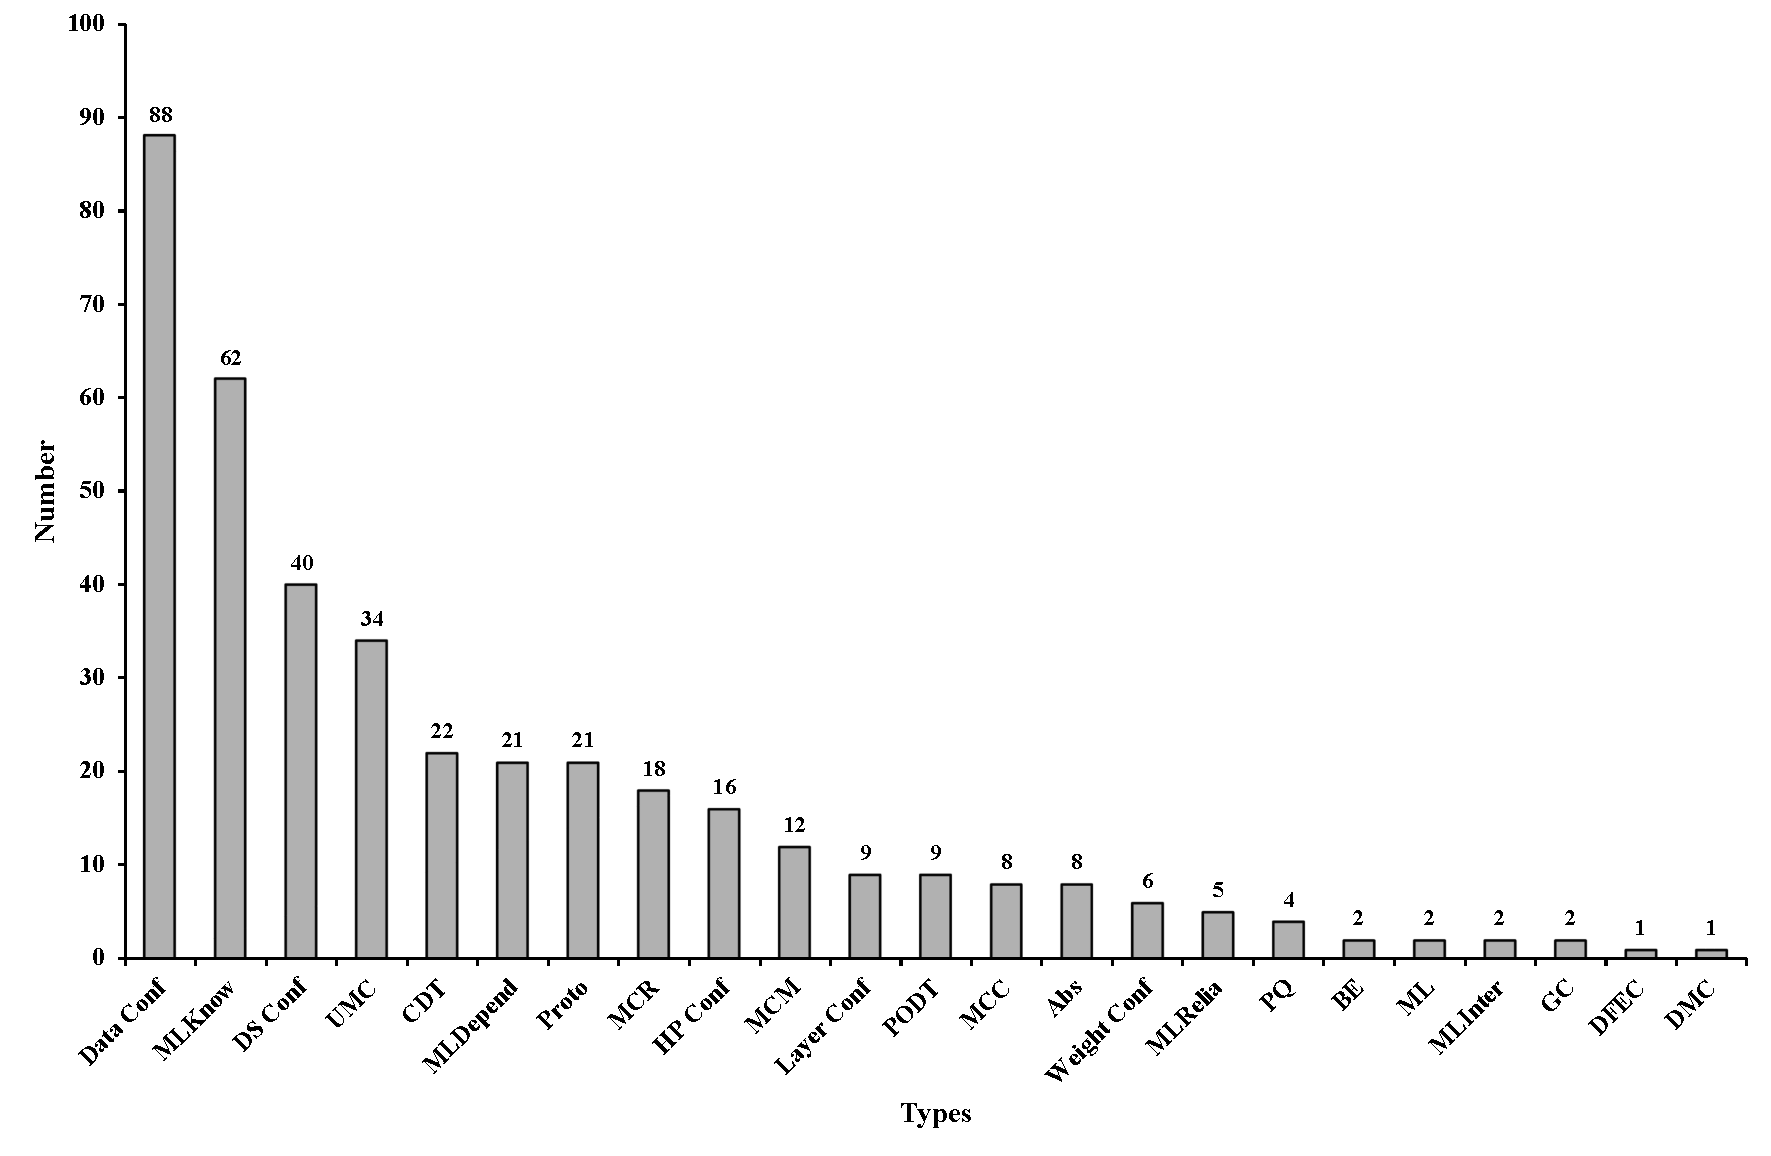
\includegraphics[width=0.8\textwidth]{Statistics info new.pdf}
    \caption{Statistical info of the processed dataset.}
    \label{fig:statistic_info}
\end{figure}

\subsection{Models}
To evaluate the effectiveness of \emph{general-purpose} and \emph{code-oriented} LLMs for fine-grained ML-SATD classification, we select models from three widely used open-weight families, namely Qwen, Gemma, and Llama, and additionally include the recently released open-weight GPT-oss model. Concretely, our evaluated models include Qwen3-8B, Qwen3-14B, Qwen2.5-Coder-7B-Instruct, gemma-2-9b-it, gemma-3-12b-it, codegemma-1.1-7b-it, Llama-3.1-8B-Instruct, CodeLlama-7b-Instruct-hf, and gpt-oss-20b. This selection enables a controlled comparison between general LLMs and code-specialized LLMs under similar parameter scales, and supports reproducibility by relying on open-weight checkpoints.

\noindent\textbf{Qwen3 series.}
Qwen3 \cite{yang2025qwen3} is the latest generation of the Qwen model family, providing both dense and Mixture-of-Experts (MoE) variants across a wide range of scales and emphasizing strong reasoning and multilingual coverage. A key design is the unified support of \emph{thinking} and \emph{non-thinking} modes, allowing the model to trade off reasoning depth and efficiency via an adjustable budget mechanism. In our experiments, we use the instruction-tuned dense variants Qwen3-8B and Qwen3-14B.

\noindent\textbf{Qwen2.5-Coder.}
Qwen2.5-Coder \cite{hui2024qwen2} is a code-specific model family built upon the Qwen2.5 architecture and further pretrained on large-scale code-centric corpora (over trillions of tokens), aiming to improve code generation and code reasoning while preserving general and mathematical abilities. We include Qwen2.5-Coder-7B-Instruct to represent a strong open code LLM at a moderate scale.

\noindent\textbf{Gemma 2 series.}
Gemma 2 \cite{team2024gemma} is a family of open-weight, decoder-only Transformer models (2B--27B) that improves efficiency and long-context modeling by interleaving local and global attention and adopting grouped-query attention. Smaller variants (including 9B) are trained with distillation to achieve competitive performance at practical sizes. We evaluate gemma-2-9b-it as the general instruction-tuned representative from this family.

\noindent\textbf{Gemma 3 series.}
Gemma 3 \cite{team2025gemma} extends the Gemma family with longer context support (at least 128K tokens) and improved multilingual capabilities, and it is trained with distillation and a revised post-training recipe to enhance instruction following and reasoning. We use gemma-3-12b-it as a newer generation general instruction-tuned model with a comparable parameter scale to other backbones in our study.

\noindent\textbf{CodeGemma.}
CodeGemma \cite{team2024codegemma} is a collection of open code models built on top of Gemma, further trained on large code-heavy corpora to strengthen code understanding and generation. We include the instruction-tuned codegemma-1.1-7b-it as the code-oriented counterpart within the Gemma ecosystem.

\noindent\textbf{Llama 3.1 series.}
Llama 3.1 \cite{grattafiori2024llama} is an open foundation model family optimized for multilingual understanding, reasoning, and coding. It is trained on large-scale high-quality tokens and released with instruction-tuned variants for interactive use. We evaluate Llama-3.1-8B-Instruct as a widely adopted open general-purpose LLM baseline.

\noindent\textbf{CodeLlama.}
CodeLlama \cite{roziere2023code} is a family of code-specialized models derived from Llama, designed for code generation and infilling, and provided with instruction-following variants for programming tasks. We include CodeLlama-7b-Instruct-hf to study whether code specialization in the Llama ecosystem benefits ML-SATD classification.

\noindent\textbf{gpt-oss-20b.}
gpt-oss-20b \cite{agarwal2025gpt} is an open-weight decoder-only Mixture-of-Experts model designed for efficient reasoning and tool use, and released with an instruction-tuned chat format that supports adjustable reasoning effort. We include gpt-oss-20b to compare a recent open-weight MoE backbone against mainstream dense open models under the same evaluation protocol.

\noindent

Overall, by evaluating both general and code-oriented backbones across multiple open model families, our study provides practical guidance on whether (and when) code specialization influences ML-SATD classification performance. For all tested models, we use the default settings and set all temperatures to zero for reproducibility.


\subsection{Evaluation Metrics}
\label{subsec:evaluation_metrics}

Following prior work on SATD classification~\cite{huang2018identifying}, we evaluate our models using precision (P), recall (R), and F1-score. In the multi-class setting, each SATD category $c_k$ is treated as a separate class. For each class $c_k$, we define the following quantities based on the multiclass confusion matrix:
\begin{itemize}
  \item $TP_k$ (true positives): the number of instances whose true label and predicted label are both $c_k$;
  \item $FP_k$ (false positives): the number of instances whose predicted label is $c_k$, but whose true label is not $c_k$;
  \item $FN_k$ (false negatives): the number of instances whose true label is $c_k$, but whose predicted label is a different class.
\end{itemize}
The class-wise precision, recall, and F1-score are then defined as:
\begin{equation}
  P_k = \frac{TP_k}{TP_k + FP_k}, \quad
  R_k = \frac{TP_k}{TP_k + FN_k}, \quad
  F1_k = \frac{2 P_k R_k}{P_k + R_k}.
\end{equation}

Since our task is multi-class and the class distribution is highly imbalanced, we report \emph{weighted averages} of precision, recall, and F1-score. Let $n_k$ be the number of test instances (support) of class $c_k$, and $N = \sum_{k=1}^{K} n_k$ be the total number of test instances. The weighted-averaged precision, recall, and F1-score are defined as:
\begin{equation}
  \text{Weighted-Precision} = \sum_{k=1}^{K} \frac{n_k}{N} P_k, \quad
  \text{Weighted-Recall}    = \sum_{k=1}^{K} \frac{n_k}{N} R_k, \quad
  \text{Weighted-}F1        = \sum_{k=1}^{K} \frac{n_k}{N} F1_k.
\end{equation}

These weighted averages correspond to the standard implementation in commonly used libraries (e.g., scikit-learn) and reflect performance under the empirical class distribution of the ML-SATD dataset.


% Among these, the F1-score
% holds particular significance as it provides a balanced assessment of the classifier’s ability to
% minimize both false positives (over-identification) and false negatives (under-identification), which
% are critical trade-offs in SATD classification tasks. In this work, we follow this convention and use
% these metrics to assess our model’s performance. The formulas for these metrics are defined as
% follows:


% TP (True Positive) denotes the number of SATDs correctly identified by the model, FP (False
% Positive) represents non-SATDs incorrectly classified as SATDs, and FN (False Negative) refers to
% SATDs misclassified as non-SATDs.



% \section{Methodology}\label{sec:methodology}

\subsection{Methodology for RQ1}

We test three different prompting strategies to identify the most effective way to instruct the LLM for fine-grained ML SATD classification: vanilla prompting, binary prompting, and hierarchical prompting. For vanilla prompting, we enumerates all target categories and instructs the model to output only one of the corresponding label abbreviation. 


The prompts used in this method are consist of two parts: 1) catergories defination. which consist of the detailed defination of the labels. 2) Task instruction. Which are the detailed instruction of different prompting.  Vanilla prompting enumerates all target categories and instructs the model to output only one of the corresponding label abbreviation. Binary prompting is a two-stage method. In the first stage, the model is asked for each type of defined ML SATD whether the given code comment belongs to that type. After this step, the model may either select multiple types or fail to select any. In the second stage, these issues are resolved: if the model returns multiple types, it is asked to choose the most likely one from the candidates; if it fails to select any, it is asked again to select from the full set of categories. Hierarchical prompting is also a two-stage method. Since the dataset contains both high-level categories and subcategories, the classification task is organized into a tree structure. The model first determines the high-level category of the ML SATD and then proceeds step by step to fine-grained subcategories until the final label is reached. 


% This can be further illustrated by adding a figure.
% Detailed prompting methods are shown in Figure~\ref{} 

% used for these three ways are shown in Figure~\ref{fig:vanilla_instructions}, Figure~\ref{fig:hierarchical_instructions} and Figure~\ref{}, and Figure~\ref{}.

% \cite{} didn't give the detailed definition of the high-level categories, so we manually write the definition and test these models under two settings, with the definition and without.




% \begin{figure}[htbp]
% \centering

% %将多个模型的输出结果输入到一个强的模型中，让它来做判断，如果不对，则让它输出一个新的


% \begin{tcolorbox}[title = {Vanilla prompting}] 

% There are 23 types of Machine Learning (ML) SATD (Self-Admitted Technical Debt):

% MACHINE LEARNING KNOWLEDGE (MLKnow): Machine-learning software carries plenty of unique challenges. Uneducated solutions by unaware developers may have to be revisited.


% MODEL INTERPRETABILITY (MLInter): Machine-learning models are a black box, causing poor understanding of model functionality; this can lead to unknown behaviour.


% MODEL CODE COMPREHENSION (MCC): Model code carries extra legibility concerns not present in traditional software (e.g., poorly-named temporary matrix variables).


% ......

% PREDICTION QUALITY (PQ): Workflow changes may affect performance.


% MACHINE LEARNING RELIABILITY (MLRelia): Model functionality depends on data quality; robustness measures should be in place.


% PROTOTYPE (Proto): Deploying small-scale prototypes into full systems can be dangerous.



% Please determine which type of ML Self-Admitted Technical Debt (SATD) the following Code Comment belongs to. 

% You MUST answer with  **only ONE**  abbreviation from:



% \end{tcolorbox}
% \caption{Example of vanilla prompting: we give the model all the categories and require the model to predict and output the abbreviation of each category.}
% \label{fig:vanilla_instructions}
% \end{figure}

% \usepackage{tabularx}

\begin{table}[ht!]
\centering
\small
\caption{Model-generated examples of the 23 Identified ML SATD Types.}
\label{tab:ml_satd_types}
\begin{tabularx}{\textwidth}{
    >{\centering\arraybackslash}p{0.8cm}
    >{\centering\arraybackslash}p{2.8cm}
    X 
}
\hline
\textbf{Dim. Name} & \textbf{Type} & \textbf{Example} \\
\hline
\multirow{4}{*}{AWR} & Machine Learning Knowledge & TODO: Confirm whether layer-norm before attention actually boosts convergence for small-batch training on this dataset \\
\cline{2-3}
 & Model Interpretability & TODO: Generate SHAP summary plot so users can see feature impact \\
\hline
\multirow{2}{*}{RDB} & Model Code Comprehension & TODO: break up monolithic function train\_eval\_predict() into clearer, single-purpose helpers \\
\hline
\multirow{4}{*}{DCE} & Duplicate Model Code & TODO: remove copy-pasted ConvBlock definition—reuse common\_layers.ConvBlock instead \\
\cline{2-3}
 & Duplicate Feature Extraction Code & XXX: text\_features\_v1 and text\_features\_v2 are copy-pasted—create one configurable pipeline \\
\hline
\multirow{6}{*}{CFO} & Weight Configuration & FIXME: pretrained checkpoint loads fp16 weights—add auto-cast to ensure dtype consistency \\
\cline{2-3}
 & Layer Configuration & TODO: swap BatchNorm for LayerNorm when depth $> 24$ \\ 
\cline{2-3}
 & Hyper-parameter Configuration & TODO: make learning\_rate schedule (cosine vs. linear) selectable via CLI flag \\
\hline
\multirow{10}{*}{CDD} & Machine Learning Dependency & TODO: bump scikit-learn to $\geq 1.6$ once conda forge wheels for arm64 become available \\  
\cline{2-3}
 & Glue Code & FIXME: adapter.py only exists to map old Predictor API to new one—rewrite consumers instead \\
\cline{2-3}
 & Custom Data Type & TODO: replace custom SparseTensorDict with standard torch.sparse\_coo\_tensor before exporting \\
\cline{2-3}
 & Multiple Languages & TODO: port custom attention kernel from CUDA C++ to Metal for macOS deployment \\
\cline{2-3}
 & Unnecessary Model Code & TODO: delete legacy compute\_grad\_stats(); superseded by torch.autograd.profiler \\
\hline
\multirow{6}{*}{DTD} & Data Processing Configuration & TODO: add configurable pipeline step to down-sample majority class before batching \\
\cline{2-3}
 & Plain Old Data Type & TODO: replace raw list of logits with a NamedTuple so callers know the order \\
\cline{2-3}
 & Data Storage Configuration & TODO: migrate checkpoint format from .pth to safetensors for safer serialization \\
\hline
\multirow{8}{*}{MDL} & Abstraction & TODO: extract common scoring logic into BaseMetric so each model wrapper isn’t re-implementing it \\
\cline{2-3}
 & Boundary Erosion & TODO: migrate training-time logging out of Trainer class; should live in metrics.logger \\
\cline{2-3}
 & Model Code Modifiability & TODO: move hyper-parameter defaults into config file so changing them doesn’t require code edits \\
\cline{2-3}
 & Model Code Reusability & TODO: abstract make\_encoder() so VisionTransformer and ResNet builders share the same backbone factory \\
\hline
\multirow{4}{*}{PRF} & Prediction Quality & TODO: rerun validation after enabling mixed-precision; confirm accuracy isn’t degraded \\
\cline{2-3}
 & Machine Learning Reliability & TODO: add sanity-check to reject examples with $> 20\%$ missing features before prediction \\
\hline
\multirow{2}{*}{SCL} & Prototype & TODO: replace the single-threaded demo server with a production-ready Gunicorn setup \\
\hline
\end{tabularx}
\end{table}

\subsection{Methodology for RQ2}\label{sec:RQ2}



Few-shot examples can improve models' performance in other tasks, however, Due to the limited size of the dataset in this task, some categories contain only a single instance, which makes it difficult to devide the dataset and select representative examples. In this RQ, we aim to test whether the model generated examples can improve the results. We use an LLM to generate additional examples. Specifically, we provide the LLM with detailed category descriptions and real word examples to prompt these LLMs to generate high-quailty examples. Then we manually verified the quaility of these generated examples, we focus on two aspect, 1) to avoid data leakage, make the generated examples is not too similar to the test case, we using the 2) to ensure the diversitries, we manually drop some generated examples are too similarly to other examples in the generated examples set. 


up to five real examples per category—using fewer examples if fewer than five instances exist—and instruct it to generate similar examples. 


\subsubsection{Model Choice.} We adopt GPT-5, a state-of-the-art model, in deep research mode to generate these examples. We generate ten synthetic examples for each category and incorporate them into the instruction. We provide an example for each category in Table \ref{tab:ml_satd_types}. It should be noted that the generated examples are fixed for each instance during inference. To examine the impact of the number of examples, we evaluate settings with 1, 2, 3, 5, and 10 examples. We incorporate these examples into the two best performing prompts found in RQ1.


\subsubsection{Examples Selection.} After get the model generated examples, we manually verified and selected the examples, we find for most of the catergories, GPT-5 can generate suitable examples, but for the generated examples some are very similar, for this situation, we using GPT-5 to regenerate it again, all the examples are different in the second generation.

After get the generate examples, we matain 10 examples of each categories and 




% \begin{figure}[t]
% \centering

% \begin{tcolorbox}[title = {CoT}] 

% You are a strict ML-SATD classifier.

% Decide the single best label by following this internal decision process, then output exactly ONE abbreviation on a single line with nothing else.

% Internal decision process (for your internal use only; do not include in output):

% 1) Identify the primary signal in the comment and select candidates accordingly:

% \begin{itemize}
%   \item \textbf{Data-related:} processing/pipeline steps \(\Rightarrow\) \{\{Data Conf\}\}; raw/plain data types \(\Rightarrow\) \{\{PODT\}\}; representation/storage/schema \(\Rightarrow\) \{\{DS Conf\}\}.
  
%   \item \textbf{Dependency \& integration:} external/library blocking \(\Rightarrow\) \{\{MLDepend\}\}; glue/integration shims \(\Rightarrow\) \{\{GC\}\}; custom data types \(\Rightarrow\) \{\{CDT\}\}; mixed languages \(\Rightarrow\) \{\{ML\}\}; unnecessary/dead/deprecated model code \(\Rightarrow\) \{\{UMC\}\}.
  
%   \item \textbf{Configuration \& parameters:} weights \(\Rightarrow\) \{\{Weight Conf\}\}; layers/topology \(\Rightarrow\) \{\{Layer Conf\}\}; hyper-parameters/defaults \(\Rightarrow\) \{\{HP Conf\}\}.
  
%   \item \textbf{Structure \& evolvability:} missing abstraction \(\Rightarrow\) \{\{Abs\}\}; boundary erosion \(\Rightarrow\) \{\{BE\}\}; ease of modifying model code \(\Rightarrow\) \{\{MCM\}\}; generality/reuse \(\Rightarrow\) \{\{MCR\}\}.
  
%   \item \textbf{Duplication:} model code duplication \(\Rightarrow\) \{\{DMC\}\}; feature-extraction duplication \(\Rightarrow\) \{\{DFEC\}\}.
  
%   \item \textbf{Understanding \& interpretability:} lack of ML knowledge \(\Rightarrow\) \{\{MLKnow\}\}; model black-box / explainability concerns \(\Rightarrow\) \{\{MLInter\}\}.
  
%   \item \textbf{Performance \& robustness:} prediction quality/accuracy \(\Rightarrow\) \{\{PQ\}\}; reliability/robustness/data-quality guards \(\Rightarrow\) \{\{MLRelia\}\}.
  
%   \item \textbf{Prototype:} prototype used beyond its scope \(\Rightarrow\) \{\{Proto\}\}.
% \end{itemize}
   
% 2) If multiple candidates match, choose the one that represents the main maintenance obstacle implied by the comment.

% 3) If still tied, prefer the most specific label whose remediation is the most localized (e.g., pick {{Layer Conf}} over {{HP Conf}} if the text explicitly mentions layers).

% 4) Output policy: return exactly ONE abbreviation on a single line, with no other text.

%    Allowed abbreviations:
%    {', '.join(sorted(ABBR\_SET))}

% \end{tcolorbox}
% \caption{Details of Chain-of-Thought instructions used in the experiments.}
% \label{sample_instructions}
% \end{figure}


\begin{figure}[t]
\centering
\begin{lstlisting}[style=cotlisting]
You are a strict ML-SATD classifier.

Decide the single best label by following this internal decision process, then output exactly ONE abbreviation on a single line with nothing else.

Internal decision process (for your internal use only; do not include in output):

1) Identify the primary signal in the comment and select candidates accordingly:

- Data-related: processing/pipeline steps => {{Data Conf}}; raw/plain data types => {{PODT}}; representation/storage/schema => {{DS Conf}}.
- Dependency & integration: external/library blocking => {{MLDepend}}; glue/integration shims => {{GC}}; custom data types => {{CDT}}; mixed languages => {{ML}}; unnecessary/dead/deprecated model code => {{UMC}}.
- Configuration & parameters: weights => {{Weight Conf}}; layers/topology => {{Layer Conf}}; hyper-parameters/defaults => {{HP Conf}}.
- Structure & evolvability: missing abstraction => {{Abs}}; boundary erosion => {{BE}}; ease of modifying model code => {{MCM}}; generality/reuse => {{MCR}}.
- Duplication: model code duplication => {{DMC}}; feature-extraction duplication => {{DFEC}}.
- Understanding & interpretability: lack of ML knowledge => {{MLKnow}}; model black-box / explainability concerns => {{MLInter}}.
- Performance & robustness: prediction quality/accuracy => {{PQ}}; reliability/robustness/data-quality guards => {{MLRelia}}.
- Prototype: prototype used beyond its scope => {{Proto}}.

2) If multiple candidates match, choose the one that represents the main maintenance obstacle implied by the comment.

3) If still tied, prefer the most specific label whose remediation is the most localized (e.g., pick {{Layer Conf}} over {{HP Conf}} if the text explicitly mentions layers).

4) Output policy: return exactly ONE abbreviation on a single line, with no other text.

Example output: Data Conf
Allowed abbreviations: Abs, BE, CDT, Data Conf, DFEC, DMC, DS Conf, GC, HP Conf, Layer Conf, MCC, MCM, MCR, ML, MLDepend, MLInter, MLKnow, MLRelia, PODT, PQ, Proto, UMC, Weight Conf

\end{lstlisting}
\caption{Details of Chain-of-Thought instructions used in the experiments.}
\label{sample_instructions}
\end{figure}


\subsection{Methodology for RQ3}\label{sec:RQ3}

To test the models' ability under thinking mode, Qwen series and GPT-OSS-20b are designed for thinking capability, so to test these models, we set these models according to the guidelines on the website to complete this task. For the Qwen series, we set \textit{enable\_thinking} equal to true. For GPT-OSS-20b, we evaluate our task under high mode which the high mode delivers deep and comprehensive analysis. 



We first compared the Qwen series under different settings which is thinking and no-thinking mode to figure out the effectiveness of thinking of these models.

We want to know whether the manually written Chain-of-Thought can improve the performance, so we first define the patterns in ML piplines to map the detailed patterns to the detailed sub catergoies. This information can give a detailed information about how these 

The thinking models We also compared the reasoning mode with the zero-shot Chain-of-Thought~\cite{kojima2022large}, which requires the model to think step by step. 


The Qwen series can be  

Previous models, which didn't include the thinking mode, were tested under chain-of-thought settings and compared with those models under the thinking mode. The thinking models are We also test the reasoning mode under chain-of-thought prompting in two steps, the first one following traditional zero-shot prompting requires model to think step by step and output reasoning and the answers. Beside the traditional zero-shot prompting, we refine these prompts by adding more detailed chain of reasoning, we manually defined the features which will lead to reason about each types. We test these refined Chain-of-thought prompting and analysis the thinking models between the chat models.




% \subsection{Methodology for RQ4}\label{sec:RQ4}

% To explore how well these models can perform on this task, we conducted a detailed analysis of the results obtained in the previous RQs and selected the best-performing models to further improve their performance by combining the prompting strategies used earlier. To identify the most promising models, we first selected the top-performing model from each family by comparing the general-purpose and code-specific variants under various prompting settings. Based on these findings, we applied the selected model types in subsequent experiments. We then evaluated the reasoning approach using examples from RQ2 and examined its effectiveness under the best-performing prompting settings derived from RQ1. Through this process, we aim to further demonstrate how to effectively prompt LLMs for the fine-grained ML SATD classification task and identify the optimal performance of these models. Based on these results, we further analyzed the size of the impact of these results and the best-performing model for this task.

\subsection{Methodology for RQ4}
\label{sec:RQ4}

RQ4 aimed to examine the overall effectiveness of LLMs on the fine-grained ML SATD classification task after combining the effective prompting strategies identified in the previous RQs. To this end, we conducted an additional round of experiments based on the results of RQ1--RQ3, to explore whether different prompting strategies combinations could further improve model performance.

We first reviewed the results obtained in the previous RQs and selected the three most promising models for further analysis. The selection was based on their overall performance under different prompting settings, including the prompt formulations studied in RQ1, the example-based settings explored in RQ2, and the reasoning strategies examined in RQ3. Rather than including all evaluated models, we focused on a smaller set of representative and competitive models in order to more clearly assess the effect of combining prompting strategies.

Based on the findings of the previous RQs, we then constructed the combined settings used in this RQ. Specifically, we adopted the best-performing prompt setting identified in RQ1 as the basis of the final experiments. On top of this setting, we incorporated the automatically generated examples investigated in RQ2 and the manually written chain-of-thought explored in RQ3. This design allowed us to evaluate whether the improvements observed in earlier RQs could be accumulated when these strategies were applied together.

In addition to the LLM-based settings, we included two simple baselines to better contextualize the final results. The first baseline was a random-guess baseline, which assigned one of the 23 ML-SATD labels uniformly at random to each instance. Since this baseline was stochastic, we repeated it 10 times with different random seeds and reported the average results together with the standard deviation. The second baseline was a majority-class baseline, which always predicted the most frequent label in the dataset. Both baselines were evaluated on the same dataset using the same weighted precision, weighted recall, and weighted F1-score as the LLM-based approaches.

The analysis in RQ4 focused on three aspects. First, we compared the LLM-based approaches with the two baselines in order to assess whether prompted LLMs could outperform simple non-LLM prediction strategies. Second, we examined whether combining prompting strategies led to further improvements over the individual settings studied in RQ1--RQ3. Third, we identified the best-performing model and prompting strategies among all evaluated settings, thereby providing a clearer picture of the performance that current LLMs can achieve on fine-grained ML SATD classification.


% To assess the current state of large language models on fine-grained ML SATD classification, we first evaluate them under a vanilla prompting setting. The prompt enumerates all target categories and instructs the model to output only the corresponding label abbreviation. In this setup, we evaluate nine models—covering both general-purpose and code-oriented LLMs—with diverse architectures and parameter scales. Their results are then compared against two baselines: random guessing and majority-class prediction, which selects the most frequent label in the dataset. We further analyze the models’ performance relative to these baselines.



% \begin{figure}[ht]
% \centering


% \begin{tcolorbox}[title = {Hierarchical prompting for the father labels}] 
% There are 9 coarse-grained types of ML SATD:

% Awareness (AWR): Lack of developer understanding or certainty about ML algorithms, APIs, data, or model behavior. Often arises due to “black box” nature of ML models.


% Readability (RDB):Model code has poor legibility or unclear logic, especially in ML contexts (e.g., poorly named variables, dense math code).


% ······

% Performance (PRF): Performance or robustness is insufficient, requiring evaluation, optimization, or reliability improvements.


% Scalability (SCL): Prototype-level code is used in production without scaling optimizations.


% Please classify the following Code Comment into exactly ONE of these coarse abbreviations:

% AWR, RDB, ······ PRF, SCL



% Return the abbreviation only (e.g., AWR).  

% \end{tcolorbox}
% \caption{Prompts used for hierarchical methods to classify the father labels.}
% \label{fig:hierarchical_instructions}
% \end{figure}

% \begin{figure}[ht]
% \centering

% %加入一个examples的表，来给出模型生成的每种类型的examples

% \begin{tcolorbox}[title = {Hierarchical prompting for the child labels}] 
% There are 23 types of Machine Learning (ML) SATD (Self-Admitted Technical Debt):

% MACHINE LEARNING KNOWLEDGE (MLKnow): Machine-learning software carries plenty of unique challenges. Uneducated solutions by unaware developers may have to be revisited.


% MODEL INTERPRETABILITY (MLInter): Machine-learning models are a black box, causing poor understanding of model functionality; this can lead to unknown behaviour.


% MODEL CODE COMPREHENSION (MCC): Model code carries extra legibility concerns not present in traditional software (e.g., poorly-named temporary matrix variables).

% ......

% PREDICTION QUALITY (PQ): Workflow changes may affect performance.


% MACHINE LEARNING RELIABILITY (MLRelia): Model functionality depends on data quality; robustness measures should be in place.


% PROTOTYPE (Proto): Deploying small-scale prototypes into full systems can be dangerous.


% Please determine the fine-grained ML SATD type. You MUST answer with only ONE abbreviation from: 

% MLKnow, MLInter, MCC, ...... PQ, MLRelia, Proto

% Return the abbreviation only (e.g., HP Conf).

% \end{tcolorbox}
% \caption{Prompt used for hierarchical approach to classify the child labels.}
% \label{sample_instructions}
% \end{figure}






% \begin{figure}[htbp]
% \centering


% \begin{tcolorbox}[title = {Binary prompting for each categories}] 
% There are 23 types of Machine Learning (ML) SATD (Self-Admitted Technical Debt):

% MACHINE LEARNING KNOWLEDGE (MLKnow): Machine-learning software carries plenty of unique challenges. Uneducated solutions by unaware developers may have to be revisited.


% MODEL INTERPRETABILITY (MLInter): Machine-learning models are a black box, causing poor understanding of model functionality; this can lead to unknown behaviour.


% MODEL CODE COMPREHENSION (MCC): Model code carries extra legibility concerns not present in traditional software (e.g., poorly-named temporary matrix variables).


% ......

% PREDICTION QUALITY (PQ): Workflow changes may affect performance.


% MACHINE LEARNING RELIABILITY (MLRelia): Model functionality depends on data quality; robustness measures should be in place.


% PROTOTYPE (Proto): Deploying small-scale prototypes into full systems can be dangerous.

% We are classifying the following code comment into one of the ML SATD categories.
        
% Code Comment: """  \{comment\}""" 

% Question: Does this comment indicate the category \{full\_label\} (\{abbr\})?
        
% Answer strictly with Yes or No.


% \end{tcolorbox}
% \caption{Example of binary prompting: we ask these models to decide whether each comment belongs to this category or not.}
% \label{sample_instructions}
% \end{figure}





\section{Results}\label{sec:results}


\subsection{RQ1: How to prompt LLMs for fine-grained ML SATD classification?}

\paragraph{Results of different prompting strategies} We compare the three prompting methods introduced above, and report the detailed zero-shot results in Table~\ref{tab:zero-shot}.

Under the vanilla prompt, gpt-oss-20b achieves the best overall performance with an F1 score of 34.0\% (precision 0.434, recall 0.344). Qwen3-14B ranks second (30.2\% F1), while gemma-3-12b places third (28.9\% F1). Overall, the vanilla setting yields relatively balanced precision-recall trade-offs for the top performance models.


With the binary prompt, performance generally improves over vanilla for most models. gpt-oss-20b remains the top model and further increases its performance to 35.1\% F1 (precision 0.397, recall 0.354). gemma-3-12b becomes the second-best model with 32.6\% F1, followed by Qwen2.5-Coder-7B-Instruct with 31.1\% F1. This may be because the binary prompting gives the LLMs a second chance to select the more precise results from the smaller candidate pools, which makes some model performance better.


For the hierarchical prompt, we observe a clear decline in overall results compared to the other two prompting strategies. Although some models obtain higher precision (e.g., gemma-2-9b reaches 0.460 precision), recall drops sharply across most models, leading to lower F1 scores. gpt-oss-20b still performs best with 32.6\% F1, but the gap to the remaining models narrows, with Qwen3-14B at 25.1\% F1 and gemma-2-9b at 23.9\% F1. These results indicate that, in a zero-shot setting, hierarchical decomposition can introduce additional error propagation across stages, making the overall prediction less accurate than the simpler vanilla or binary prompts.


\paragraph{Summary of different prompting strategies}


Among the nine models evaluated, the vanilla prompting and binary classification prompting achieve comparable performance, while the hierarchical prompting performs the worst. Comparing the vanilla and hierarchical prompting approaches, we find that eight out of nine models perform better in terms of F1 score under the vanilla setting. A similar trend is observed for the binary prompting, where all models outperform those using the hierarchical approach. We attribute this to the difficulty LLMs face in understanding higher-level hierarchical labels, which may lead to error accumulation when predicting the final results, ultimately degrading performance. Comparing the vanilla prompting with the binary prompting, we find that these two approaches yield comparable performance, with the binary approach performing slightly better. Specifically, six out of nine models perform better under the binary setting than under the vanilla one. We believe this is because both approaches do not introduce additional information that could increase the model’s cognitive burden. Moreover, the binary approach allows the model to group uncertain types and provides a second opportunity to make a more accurate prediction.


\paragraph{Error analysis} We provide detailed analysis of the hierarchical prompting 



% \paragraph{Error analysis}
% We further give a detailed analysis of the 


\begin{table}[htbp]
  \centering
  \caption{Zero-shot results on three prompting methods}
  \label{tab:zero-shot}
  \setlength{\tabcolsep}{6pt}
  \renewcommand{\arraystretch}{1.15}
  % Force the table to fit the text width
  \resizebox{\textwidth}{!}{%
  \begin{tabular}{l*{9}{c}}
    \toprule
    \multirow{2}{*}{Model} &
      \multicolumn{3}{c}{Vanilla} &
      \multicolumn{3}{c}{Binary} &
      \multicolumn{3}{c}{Hierarchical} \\
    \cmidrule(lr){2-4}\cmidrule(lr){5-7}\cmidrule(lr){8-10}
    & precision & recall & f1
    & precision & recall & f1
    & precision & recall & f1 \\
    \midrule
    Qwen3-8B                 & 0.210 & 0.196 & 0.168 & 0.315 & 0.237 & 0.249 & 0.263 & 0.198 & 0.170 \\
    Qwen3-14B                & 0.379 & 0.305 & 0.302 & 0.387 & 0.280 & 0.284 & 0.452 & 0.244 & 0.251 \\
    Qwen2.5-Coder-7B-Instruct& 0.315 & 0.262 & 0.242 & 0.406 & 0.323 & 0.311 & 0.398 & 0.221 & 0.210 \\
    gemma-2-9b               & 0.370 & 0.290 & 0.268 & \textbf{0.407} & 0.293 & 0.279 & \textbf{0.460} & 0.270 & 0.239 \\
    gemma-3-12b              & 0.412 & 0.285 & 0.289 & 0.404 & 0.328 & 0.326 & 0.309 & 0.272 & 0.228 \\
    codegemma-1.1-7b-it      & 0.308 & 0.198 & 0.167 & 0.291 & 0.183 & 0.171 & 0.296 & 0.094 & 0.083 \\
    Llama-3.1-8B-Instruct    & 0.231 & 0.221 & 0.156 & 0.301 & 0.153 & 0.146 & 0.219 & 0.089 & 0.095 \\
    CodeLlama-7b-Instruct-hf & 0.214 & 0.148 & 0.108 & 0.109 & 0.048 & 0.052 & 0.077 & 0.028 & 0.017 \\
    gpt-oss-20b              & \textbf{0.434} & \textbf{0.344} & \textbf{0.340} & 0.397 & \textbf{0.354} & \textbf{0.351} & 0.434 & \textbf{0.310} & \textbf{0.326} \\
    \bottomrule
  \end{tabular}%
  }
\end{table}



\begin{boxB}
\textbf{Findings:} (1) For fine-grained ML SATD classification, the vanilla prompting and the binary prompting achieve similar results, and the hierarchical prompting is the worst. 

(2) GPT-oss-20b under the binary prompting setting is the best model for fine-grained ML SATD classification under zero-shot settings.


\end{boxB}


\subsection{RQ2: Can incorporating LLM-generated examples improve the performance of LLMs on fine-grained ML SATD classification?}



We add the examples into two prompting strategies which are  were revealed in RQ1, that is Vanilla prompting and Binary prompting.

\paragraph{Overall effectiveness of adding examples}



Incorporating LLM-generated examples can improve performance. The detailed results are shown in Table~\ref{tab:vanilla_few_shot} and Table~\ref{tab:binary_few_shot}. Compared with the zero-shot results on this task, under the vanilla prompting setting, we find that all models achieve better results than in the zero-shot setting. The same trend is also observed under the binary prompting setting, where seven out of nine models perform better than in the zero-shot setting.



Under the vanilla prompting, adding LLM-generated examples is beneficial for most models. Specifically, 7 out of 9 models achieve a higher F1 score when providing one or more examples than in the zero-shot setting, indicating that adding examples is generally effective. Among them, Qwen3-8B shows the largest improvement, with its F1 score increasing from 16.8\% in the zero-shot setting to 25.6\% with 5 examples, yielding an absolute gain of 8.8\%. The second- and third-largest improvements are observed for Llama-3.1-8B-Instruct and codegemma-1.1-7b-it, whose F1 scores improve by 6.7\% and 5.3\%, respectively. In contrast, Qwen2.5-Coder-7B-Instruct and gemma-3-12b do not benefit from adding examples, as none of their few-shot results surpass their corresponding zero-shot performance. In terms of the best overall performance achieved under this setting, the top three models are gpt-oss-20b, which achieves the highest F1 score of 36.9\% with 2 examples, followed by Qwen3-14B with 33.8\% at 3-shot, and gemma-2-9b with 29.8\% at 2-shot.



\begin{table}[th!]
  \centering
  \caption{Few-shot result under the vanilla prompting setting}
  \label{tab:vanilla_few_shot}
  \setlength{\tabcolsep}{4pt}
  \renewcommand{\arraystretch}{1.15}
  
  \resizebox{\textwidth}{!}{%
  \begin{tabular}{
    >{\centering\arraybackslash}p{1cm}
    >{\centering\arraybackslash}p{1.2cm}
    *{10}{>{\centering\arraybackslash}p{1.9cm}}
  }
    \toprule
    & & Qwen3-8B & Qwen3-14B & Qwen2.5-Coder-7B-Instruct & gemma-2-9b & gemma-3-12b & codegemma-1.1-7b-it & Llama-3.1-8B-Instruct & CodeLlama-7b-Instruct-hf & gpt-oss-20b \\
    \midrule
    % --- 0-shot ---
    \multirow{3}{*}{0} & precision & 0.210 & 0.379 & 0.315 & 0.370 & 0.412 & \textbf{0.308} & 0.231 & \textbf{0.214} & \textbf{0.434} \\
    & recall & 0.196 & 0.305 & \textbf{0.262} & 0.290 & 0.285 & 0.198 & 0.221 & 0.148 & 0.344 \\
    & f1 & 0.168 & 0.302 & \textbf{0.242} & 0.268 & \textbf{0.289} & 0.167 & 0.156 & 0.108 & 0.340 \\
    \midrule
    % --- 1-shot ---
    \multirow{3}{*}{1} & precision & 0.246 & 0.388 & 0.294 & 0.337 & 0.407 & 0.256 & \textbf{0.298} & 0.186 & 0.397 \\
    & recall & 0.232 & 0.275 & 0.244 & \textbf{0.310} & \textbf{0.303} & 0.229 & 0.214 & 0.142 & 0.356 \\
    & f1 & 0.208 & 0.287 & 0.230 & 0.275 & 0.263 & 0.195 & 0.189 & \textbf{0.140} & 0.346 \\
    \midrule
    % --- 2-shot ---
    \multirow{3}{*}{2} & precision & 0.256 & 0.419 & 0.297 & \textbf{0.378} & 0.401 & 0.284 & 0.237 & 0.189 & 0.431 \\
    & recall & 0.249 & 0.313 & 0.229 & 0.303 & 0.295 & \textbf{0.265} & 0.206 & 0.183 & \textbf{0.379} \\
    & f1 & 0.238 & 0.328 & 0.213 & \textbf{0.298} & 0.260 & \textbf{0.220} & 0.191 & 0.123 & \textbf{0.369} \\
    \midrule
    % --- 3-shot ---
    \multirow{3}{*}{3} & precision & 0.255 & \textbf{0.422} & \textbf{0.345} & 0.359 & \textbf{0.435} & 0.243 & 0.270 & 0.126 & 0.415 \\
    & recall & 0.260 & \textbf{0.321} & 0.234 & 0.298 & 0.275 & 0.237 & \textbf{0.226} & 0.186 & 0.344 \\
    & f1 & 0.234 & \textbf{0.338} & 0.231 & 0.278 & 0.234 & 0.195 & \textbf{0.223} & 0.124 & 0.345 \\
    \midrule
    % --- 5-shot ---
    \multirow{3}{*}{5} & precision & \textbf{0.302} & 0.368 & 0.293 & 0.355 & 0.406 & 0.251 & 0.250 & 0.144 & 0.402 \\
    & recall & \textbf{0.280} & 0.272 & 0.209 & 0.277 & 0.282 & 0.201 & 0.196 & 0.168 & 0.344 \\
    & f1 & \textbf{0.256} & 0.287 & 0.210 & 0.268 & 0.247 & 0.184 & 0.189 & 0.107 & 0.348 \\
    \midrule
    % --- 10-shot ---
    \multirow{3}{*}{10} & precision & 0.254 & 0.370 & 0.298 & 0.298 & 0.205 & 0.252 & 0.270 & 0.050 & 0.427 \\
    & recall & 0.224 & 0.277 & 0.204 & 0.234 & 0.226 & 0.191 & 0.201 & \textbf{0.224} & 0.349 \\
    & f1 & 0.222 & 0.287 & 0.206 & 0.220 & 0.170 & 0.158 & 0.185 & 0.082 & 0.352 \\
    \bottomrule
  \end{tabular}%
  }
\end{table}
\begin{table}[t!]
  \centering
  \caption{Few-shot result under the binary prompting setting}
  \label{tab:binary_few_shot}
  \setlength{\tabcolsep}{4pt}
  \renewcommand{\arraystretch}{1.15}
  
  \resizebox{\textwidth}{!}{%
  \begin{tabular}{
    >{\centering\arraybackslash}p{1cm}
    >{\centering\arraybackslash}p{1.2cm}
    *{10}{>{\centering\arraybackslash}p{1.9cm}}
  }
    \toprule
    & & Qwen3-8B & Qwen3-14B & Qwen2.5-Coder-7B-Instruct & gemma-2-9b & gemma-3-12b & codegemma-1.1-7b-it & Llama-3.1-8B-Instruct & CodeLlama-7b-Instruct-hf & gpt-oss-20b \\
    \midrule
    % --- 0-shot ---
    \multirow{3}{*}{0} & precision & 0.315 & 0.387 & \textbf{0.406} & 0.407 & \textbf{0.404} & 0.291 & 0.301 & 0.109 & 0.397 \\
    & recall & 0.237 & 0.280 & \textbf{0.323} & 0.293 & 0.328 & 0.183 & 0.153 & 0.048 & 0.354 \\
    & f1 & 0.249 & 0.284 & \textbf{0.311} & 0.279 & \textbf{0.326} & 0.171 & 0.146 & 0.052 & 0.351 \\
    \midrule
    % --- 1-shot ---
    \multirow{3}{*}{1} & precision & 0.316 & 0.399 & 0.333 & 0.404 & 0.404 & \textbf{0.379} & 0.276 & 0.138 & \textbf{0.412} \\
    & recall & 0.265 & 0.282 & 0.298 & \textbf{0.300} & \textbf{0.338} & \textbf{0.234} & \textbf{0.211} & 0.061 & \textbf{0.356} \\
    & f1 & 0.258 & 0.302 & 0.282 & \textbf{0.312} & 0.324 & \textbf{0.218} & 0.203 & 0.067 & \textbf{0.357} \\
    \midrule
    % --- 2-shot ---
    \multirow{3}{*}{2} & precision & \textbf{0.352} & \textbf{0.456} & 0.354 & 0.416 & 0.383 & 0.281 & 0.369 & 0.147 & 0.397 \\
    & recall & 0.267 & 0.316 & 0.321 & 0.298 & 0.326 & 0.219 & 0.209 & 0.079 & 0.351 \\
    & f1 & 0.281 & 0.335 & 0.298 & 0.309 & 0.305 & 0.190 & \textbf{0.226} & 0.075 & 0.348 \\
    \midrule
    % --- 3-shot ---
    \multirow{3}{*}{3} & precision & 0.333 & 0.449 & 0.347 & 0.416 & 0.363 & 0.232 & 0.374 & 0.270 & 0.395 \\
    & recall & \textbf{0.285} & 0.316 & 0.293 & 0.290 & 0.300 & 0.209 & 0.201 & 0.089 & 0.354 \\
    & f1 & \textbf{0.284} & 0.337 & 0.272 & 0.305 & 0.288 & 0.149 & 0.207 & 0.092 & 0.351 \\
    \midrule
    % --- 5-shot ---
    \multirow{3}{*}{5} & precision & 0.346 & 0.452 & 0.377 & \textbf{0.419} & 0.402 & 0.287 & 0.348 & \textbf{0.309} & 0.405 \\
    & recall & 0.262 & \textbf{0.318} & 0.288 & 0.277 & 0.308 & 0.224 & 0.181 & 0.097 & 0.344 \\
    & f1 & 0.267 & \textbf{0.342} & 0.286 & 0.289 & 0.309 & 0.175 & 0.184 & 0.084 & 0.341 \\
    \midrule
    % --- 10-shot ---
    \multirow{3}{*}{10} & precision & 0.340 & 0.429 & 0.264 & 0.312 & 0.397 & 0.261 & \textbf{0.379} & 0.123 & 0.381 \\
    & recall & 0.234 & 0.285 & 0.183 & 0.186 & 0.270 & 0.173 & 0.191 & \textbf{0.122} & 0.338 \\
    & f1 & 0.250 & 0.301 & 0.189 & 0.191 & 0.282 & 0.156 & 0.205 & \textbf{0.099} & 0.334 \\
    \bottomrule
  \end{tabular}%
  }
\end{table}
\begin{table}[htbp]
  \centering
  \caption{Results on coarse-grained categories under the hierarchical setting}
  \label{tab:hierarchical-coarse}
  \setlength{\tabcolsep}{6pt}
  \renewcommand{\arraystretch}{1.15}
  \begin{tabular}{lccc}
    \toprule
    Model & precision & recall & f1 \\
    \midrule
    Qwen3-8B                  & 0.405 & 0.254 & 0.214 \\
    Qwen3-14B                 & 0.517 & 0.318 & 0.350 \\
    Qwen2.5-Coder-7B-Instruct & 0.484 & 0.331 & 0.319 \\
    gemma-2-9b                & 0.519 & 0.366 & 0.364 \\
    gemma-3-12b               & 0.511 & 0.341 & 0.333 \\
    codegemma-1.1-7b-it       & 0.503 & 0.176 & 0.182 \\
    Llama-3.1-8B-Instruct     & \textbf{0.548} & 0.117 & 0.127 \\
    CodeLlama-7b-Instruct-hf  & 0.096 & 0.033 & 0.026 \\
    gpt-oss-20b               & 0.530 & \textbf{0.392} & \textbf{0.420} \\
    \bottomrule
  \end{tabular}
\end{table}

% \begin{table}[htbp]
  \centering
  \caption{Prompt settings for fine-grained ML-SATD classification}
  \label{tab:prompt-settings}
  \setlength{\tabcolsep}{6pt}
  \renewcommand{\arraystretch}{1.15}
  \resizebox{\textwidth}{!}{%
  \begin{tabular}{llllll}
    \toprule
    \textbf{Setting} & \textbf{Base Prompt} & \textbf{Examples} & \textbf{Reasoning Rule} & \textbf{Best Model} & \textbf{Weighted F1} \\
    \midrule
    Basic direct prompting              & Vanilla & 0   & No  & Qwen3-14B   & 0.341 \\
    Basic candidate-screening prompting & Binary  & 0   & No  & gpt-oss-20b & 0.351 \\
    Few-shot-enhanced prompting         & Vanilla & $2$ & No  & gpt-oss-20b & 0.369 \\
    Reasoning-enhanced prompting        & Vanilla & 0   & Yes & Qwen3-14B   & 0.363 \\
    \rowcolor{gray!15}
    Combined prompting method           & Vanilla & $3$ & Yes & Qwen3-8B    & \textbf{0.381} \\
    \bottomrule
  \end{tabular}%
  }
\end{table}
Under the binary prompting setting, adding in-context examples is also beneficial for most models. Specifically, 7 out of 9 models achieve a higher F1 score in at least one few-shot configuration than in the 0-shot setting, indicating that example augmentation remains generally effective under this prompting strategy. Among all models, Llama-3.1-8B-Instruct shows the largest improvement, with its F1 score increasing from 14.6\% in the 0-shot setting to 22.6\% with 2 examples, yielding an absolute gain of 8.0 percentage points. The second-largest improvement is observed for Qwen3-14B, whose F1 score improves from 28.4\% to 34.2\% at 5-shot, corresponding to an increase of 5.8 percentage points. codegemma-1.1-7b-it and CodeLlama-7b-Instruct-hf also show notable gains, with both improving by 4.7 percentage points over their 0-shot results. In contrast, Qwen2.5-Coder-7B-Instruct and gemma-3-12b do not benefit from adding examples, as none of their few-shot results exceed their corresponding 0-shot performance. In terms of the best overall performance achieved under this setting, the top three models are gpt-oss-20b, which attains the highest F1 score of 35.7\% with 1 example, followed by Qwen3-14B with 34.2\% at 5-shot, and gemma-3-12b with 32.6\% in the 0-shot setting.




\paragraph{Impact of number of examples}


We further analysis the impact of the numbers of examples, from Table~\ref{tab:vanilla_few_shot} and Table~\ref{tab:binary_few_shot}, we find that adding more examples into the prompts don't lead to improved performance. Under the vanilla setting, we find that most models achieve their best few-shot performance when provided with fewer than three examples. Specifically, 6 out of 9 models reach their highest F1 scores at either 1-shot or 2-shot, including Qwen2.5-Coder-7B-Instruct, gemma-2-9b, gemma-3-12b, codegemma-1.1-7b-it, CodeLlama-7b-Instruct-hf, and gpt-oss-20b. Qwen3-14B and Llama-3.1-8B-Instruct achieve their best results at 3-shot, while Qwen3-8B is the only model whose best performance appears at 5-shot. Importantly, increasing the number of examples to 10 does not further improve any model under vanilla prompting, and in most cases leads to a decline compared with the best few-shot setting. For example, gemma-2-9b drops from 29.8\% at 2-shot to 22.0\% at 10-shot, codegemma-1.1-7b-it decreases from 22.0\% to 15.8\%, and CodeLlama-7b-Instruct-hf falls from 14.0\% at 1-shot to 8.2\%.

A similar trend can also be observed under the binary prompting setting. Again, 6 out of 9 models achieve their best few-shot performance with only 1 or 2 examples, including Qwen2.5-Coder-7B-Instruct, gemma-2-9b, gemma-3-12b, codegemma-1.1-7b-it, Llama-3.1-8B-Instruct, and gpt-oss-20b. Qwen3-8B reaches its best result at 3-shot, Qwen3-14B at 5-shot, and CodeLlama-7b-Instruct-hf is the only model whose best few-shot result appears at 10-shot. However, even in this case, the overall performance remains relatively low. More importantly, larger numbers of examples are usually not helpful: for instance, gpt-oss-20b declines from 35.7\% at 1-shot to 33.4\% at 10-shot, Qwen3-14B drops from 34.2\% at 5-shot to 30.1\%, and Qwen2.5-Coder-7B-Instruct decreases substantially from 29.8\% at 2-shot to 18.9\%.

Overall, these results indicate that the performance gain from few-shot prompting is not increased with the number of examples. Across the two prompting settings, 12 out of 18 model--prompt combinations achieve their best few-shot performance with only 1 or 2 examples, and 15 out of 18 achieve their best result with no more than 3 examples. This suggests that a small number of examples is usually sufficient to provide useful task guidance, while adding too many examples may instead introduce noise and increase the cognitive burden of the model.


\begin{boxB}
\textbf{Findings:} (1)Incorporating the LLM-generated examples can improve the performance.

(2) Not incorporating more examples yields better results, and we find that adding fewer than three examples can achieve better results.


\end{boxB}


\subsection{RQ3: Can reasoning improve the performance of LLMs on fine-grained ML SATD classification?}

% Chain-of-Thought is a commonly used prompting technique in LLMs, which helps improve models’ problem-solving ability by encouraging step-by-step reasoning. This approach improves accuracy and enables LLMs to more effectively emulate human-like reasoning processes.

\paragraph{Comparison between Thinking and no-Thinking mode}


Table~\ref{tab:model_prompt_thinking} compares the effect of enabling thinking mode under both Vanilla and Binary prompting. Overall, enabling thinking consistently improves performance across all models, indicating that these reasoning model allowing them to performance deep analysis of the task and find some useful patterns to get better results beneficial for fine-grained ML-SATD classification. Under Vanilla prompting, the gains are particularly substantial. For Qwen3-8B, enabling thinking improves precision from 0.210 to 0.403, recall from 0.196 to 0.326, and F1 from 0.168 to 0.303, yielding an absolute F1 gain of 13.5 percentage points. Qwen3-14B also benefits from thinking under Vanilla prompting, with F1 increasing from 0.302 to 0.341. These results suggest that reasoning helps the model better interpret the label semantics and make more accurate decisions when the prompt.

Under Binary prompting, thinking still brings improvements, but the gains are noticeably smaller than those under Vanilla prompting. For Qwen3-8B, thinking raises F1 from 0.249 to 0.282, while for Qwen3-14B, the improvement is more limited, from 0.284 to 0.300. A closer look shows that the main benefit of thinking in the Binary setting lies in precision rather than recall. For example, Qwen3-14B improves precision from 0.387 to 0.467, but recall increases only slightly from 0.280 to 0.308. This indicates that, under Binary prompting, thinking makes the model more cautious and selective, which improves correctness of positive predictions but does not substantially expand coverage. In summary, thinking is consistently helpful, but its effect is stronger under Vanilla prompting, especially for the smaller model, suggesting that reasoning is most valuable when the prompt leaves more room for the model to structure its own decision process.


% Table 5 is tested under thinking mode. Thinking and No-thinking is the results of not adding CoT 

% Table 6 is the results tested under thinking mode, and add manually summarized CoT



\begin{table}[htbp]
  \centering
  \small
  \caption{Thinking vs No-Thinking}
  \label{tab:model_prompt_thinking}
  \setlength{\tabcolsep}{4pt}
  \renewcommand{\arraystretch}{1.15}
  \begin{tabular}{c c c c c c}
    \toprule
    \multirow{2}{*}{Models} & \multirow{2}{*}{Metric} & \multicolumn{2}{c}{Vanilla} & \multicolumn{2}{c}{Binary} \\
    \cmidrule(lr){3-4}\cmidrule(lr){5-6}
    & & no-thinking & thinking & no-thinking & thinking \\
    \midrule
    \multirow{3}{*}{Qwen3-8B} & precision & 0.210 & \textbf{0.403} & 0.315 & 0.398 \\
    & recall & 0.196 & \textbf{0.326} & 0.237 & 0.267 \\
    & f1 & 0.168 & \textbf{0.303} & 0.249 & 0.282 \\
    \midrule
    \multirow{3}{*}{Qwen3-14B} & precision & 0.379 & 0.420 & 0.387 & \textbf{0.467} \\
    & recall & 0.305 & \textbf{0.366} & 0.280 & 0.308 \\
    & f1 & 0.302 & \textbf{0.341} & 0.284 & 0.300 \\
    \bottomrule
  \end{tabular}%
\end{table}
\begin{table}[htbp]
  \centering
  \small
  \caption{Results of different models under Vanilla and Binary prompting settings}
  \label{tab:vanilla_binary_CoT}
  \setlength{\tabcolsep}{6pt}
  \renewcommand{\arraystretch}{1.15}
  \begin{tabular}{l*{6}{c}}
    \toprule
    \multirow{2}{*}{Model} &
      \multicolumn{3}{c}{Vanilla\_CoT} &
      \multicolumn{3}{c}{Binary\_CoT} \\
    \cmidrule(lr){2-4}\cmidrule(lr){5-7}
    & precision & recall & f1
    & precision & recall & f1 \\
    \midrule
    Qwen3-8B                  & 0.356 & 0.333 & 0.295 & 0.389 & 0.349 & 0.333 \\
    Qwen3-14B                 & \textbf{0.472} & \textbf{0.384} & \textbf{0.363} & 0.400 & 0.336 & 0.313 \\
    Qwen2.5-Coder-7B-Instruct & 0.351 & 0.310 & 0.289 & 0.407 & 0.316 & 0.300 \\
    gemma-2-9b                & 0.355 & 0.288 & 0.275 & 0.382 & 0.295 & 0.297 \\
    gemma-3-12b               & 0.390 & 0.285 & 0.270 & 0.381 & 0.290 & 0.292 \\
    codegemma-1.1-7b-it       & 0.394 & 0.239 & 0.218 & \textbf{0.450} & 0.244 & 0.231 \\
    Llama-3.1-8B-Instruct     & 0.213 & 0.178 & 0.141 & 0.321 & 0.155 & 0.155 \\
    CodeLlama-7b-Instruct-hf  & 0.161 & 0.102 & 0.071 & 0.135 & 0.066 & 0.065 \\
    gpt-oss-20b               & 0.427 & 0.359 & 0.345 & 0.447 & \textbf{0.372} & \textbf{0.362} \\
    \bottomrule
  \end{tabular}
\end{table}


\paragraph{Effectiveness of incorporating CoT}
Table~\ref{tab:vanilla_binary_CoT} shows the effectiveness of adding manually summarized Chain-of-Thought. Compared with the corresponding zero-shot results in Table~\ref{tab:zero-shot}, the performance of most models improves after incorporating the reasoning prompt. Under the vanilla prompting setting, 6 out of 9 models achieve higher F1 scores than in the original zero-shot setting. The largest improvement is observed for Qwen3-8B, whose F1 score increases from 16.8\% to 29.5\%, yielding an absolute gain of 12.7 percentage points. Qwen3-14B and codegemma-1.1-7b-it also show clear improvements, with F1 gains of 6.1 and 5.1 percentage points, respectively. Under the binary prompting setting, the manually written CoT is beneficial for 7 out of 9 models. Again, Qwen3-8B shows the largest improvement, with its F1 score increasing from 24.9\% to 33.3\%, followed by codegemma-1.1-7b-it, whose F1 score rises from 17.1\% to 23.1\%. These results indicate that manually written CoT is generally effective for fine-grained ML-SATD classification, especially when the task requires distinguishing highly similar labels.



Compare the Qwen series under the thinking mode and those traditional LLMs argument by the with the manually written CoT easoning prompt, we find that Qwen series model's performance increased compared to the one without thinking. Qwen3-series outperform the 

\paragraph{Case Study.} We further analysis the impact of these 



\begin{boxB}
\textbf{Findings:} (1) Reasoning mode can improve the performance, and incorporating the manually written Chain-of-thought can further improve the performance. 

(2) Reasoning models are the best choice for fine-grained ML SATD classification task; they are better than traditional models and even incorporate the manually written Chain-of-thought, it still surpasses these models.


\end{boxB}


\paragraph{Effectiveness of incorporating CoT}


Comparing the Qwen series under thinking mode with those using manually written CoT, we find that manually summarized reasoning instructions remain helpful even for reasoning-capable models. For Qwen3-14B, incorporating CoT further improves performance in both prompting settings, with F1 increasing from 34.1\% to 36.3\% under vanilla prompting and from 30.0\% to 31.3\% under binary prompting. For Qwen3-8B, manually written CoT slightly underperforms native thinking under vanilla prompting (29.5\% vs.\ 30.3\%), but leads to a much stronger result under binary prompting, where F1 increases from 28.2\% to 33.3\%. This suggests that manually summarized CoT and native thinking are not redundant; instead, they can provide complementary benefits, especially when the prompt structure constrains the reasoning process. Overall, the Qwen3-series remains among the strongest models in this setting, which further confirms that reasoning-capable models are particularly suitable for fine-grained ML-SATD classification.

\begin{boxB}
\textbf{Findings:} 
(1) Reasoning mode can improve performance, and incorporating manually written Chain-of-Thought can further improve the results for most models.

(2) Reasoning-capable models are the best choice for fine-grained ML SATD classification. Even without manually written CoT, they already outperform most traditional models, and with additional reasoning guidance, they achieve even stronger performance.
\end{boxB}



\subsection{RQ4: How effective are LLMs on fine-grained classification of ML SATD?}


\paragraph{Baseline results}

To better understand the effectiveness of LLMs on this task, we first compare them with two simple baselines, namely random guess and majority-class prediction. For the random-guess baseline, the predictor randomly selects one of the classes in the 23 label types. We repeated the experiment 10 times with different random seeds and report the average results together with the standard deviation. The random-guess baseline achieves a weighted precision of 0.109 $\pm$ 0.034, a weighted recall of 0.044 $\pm$ 0.013, and a weighted F1-score of 0.054 $\pm$ 0.016.

For the majority-class baseline, which predicts the most frequent label in the dataset, namely \textit{Data Processing Configuration}. Under this setting, the majority-class baseline achieves a weighted precision of 0.050, a weighted recall of 0.224, and a weighted F1-score of 0.082. Compared with random guessing, the majority-class baseline yields a noticeably higher recall and F1-score, which reflects the imbalanced label distribution of the dataset. 



Not all models under the different settings explored in RQ1-RQ3 outperform the random-guess baseline or the majority-class baseline. For example, CodeLlama-7b-Instruct-hf under the hierarchical prompting setting performs the worst and even falls below random guessing. This shows the importance of model selection and prompting strategies.


\paragraph{Combination results}

Table~\ref{tab:combination_results} presents the results obtained by combining the effective prompting strategies identified in the previous RQs. Overall, the results show that the combination of prompting strategies can further improve model performance on fine-grained ML SATD classification. In particular, using examples together with manually written chain-of-thought generally leads to better results than the corresponding zero-shot setting, although the improvement varies across models and prompting strategies.

Considering weighted F1-score as the main evaluation metric, the best overall result is achieved by \textbf{Qwen3-8B} under \textbf{vanilla prompting} with \textbf{three examples}, reaching an F1-score of \textbf{0.381}. This is also the highest F1-score among all settings explored in our study. The result slightly surpasses the best performance of \textbf{gpt-oss-20B}, which achieves an F1-score of 0.375 under vanilla prompting with three examples, and also exceeds the strongest binary-prompting results, where both Qwen3-8B and Qwen3-14B reach 0.377 with three examples.

The effect of adding examples is generally positive. Under vanilla prompting, the F1-score of Qwen3-8B increases steadily from 0.295 with zero examples to 0.381 with three examples, showing the largest improvement among all configurations. A similar trend can also be observed for gpt-oss-20B, whose F1-score increases from 0.355 to 0.375. Under binary prompting, Qwen3-8B improves from 0.333 to 0.377, while Qwen3-14B improves from 0.313 to 0.377. For Qwen3-14B under vanilla prompting, however, the improvement is marginal, with the best result appearing at one example (0.365), followed by a slight decline when more examples are added. These results suggest that examples are generally beneficial, but the optimal number of examples still depends on the model and prompting style.

The comparison between vanilla and binary prompting also reveals model-specific differences in the final combined setting. For Qwen3-8B and gpt-oss-20B, vanilla prompting produces the best final results when combined with three examples and manually written chain-of-thought. In contrast, Qwen3-14B performs better under binary prompting, where its best F1-score reaches 0.377. This finding indicates that the effectiveness of the final prompting combination is not determined by a single prompting style alone, but by the interaction between the model and the prompting design.

Taken together, these results suggest that the strategies explored in RQ1--RQ3 are complementary. The prompt setting identified in RQ1 provides an effective basis for the task, the examples examined in RQ2 help the models better capture fine-grained distinctions among ML-SATD labels, and the reasoning strategy studied in RQ3 further improves classification performance. By combining these strategies, we obtain the strongest results of the evaluated models on this task.


% \begin{table}[ht]
  \centering
  \caption{basic new CoT results}
  \label{tab:basic_new_CoT_results}
  \setlength{\tabcolsep}{4pt}
  \renewcommand{\arraystretch}{1.15}
  
  \resizebox{\textwidth}{!}{%
  \begin{tabular}{
    >{\centering\arraybackslash}p{1cm}
    >{\centering\arraybackslash}p{1.2cm}
    *{8}{>{\centering\arraybackslash}p{1.9cm}}
  }
    \toprule
    & & Qwen3-8B & Qwen3-14B & gemma-2-9b & gemma-3-12b & Llama-3.1-8B-Instruct & gpt-oss-20b \\
    \midrule
    % --- 0-shot ---
    \multirow{3}{*}{0} & precision & 0.356 & \textbf{0.472} & 0.355 & \textbf{0.390} & 0.213 & 0.420 \\
    & recall & 0.333 & \textbf{0.384} & 0.288 & 0.285 & 0.178 & 0.377 \\
    & f1 & 0.295 & 0.363 & 0.275 & 0.270 & 0.141 & 0.355 \\
    \midrule
    % --- 1-shot ---
    \multirow{3}{*}{1} & precision & 0.397 & 0.433 & 0.333 & 0.302 & \textbf{0.312} & 0.405 \\
    & recall & 0.359 & 0.364 & 0.321 & 0.295 & \textbf{0.224} & 0.359 \\
    & f1 & 0.345 & \textbf{0.365} & 0.292 & 0.263 & \textbf{0.219} & 0.349 \\
    \midrule
    % --- 2-shot ---
    \multirow{3}{*}{2} & precision & 0.430 & 0.438 & 0.357 & 0.323 & 0.257 & \textbf{0.441} \\
    & recall & 0.366 & 0.372 & 0.331 & \textbf{0.308} & 0.183 & 0.359 \\
    & f1 & 0.351 & 0.363 & 0.310 & 0.280 & 0.199 & 0.358 \\
    \midrule
    % --- 3-shot ---
    \multirow{3}{*}{3} & precision & \textbf{0.445} & 0.425 & \textbf{0.368} & 0.382 & 0.302 & 0.436 \\
    & recall & \textbf{0.389} & 0.361 & \textbf{0.333} & 0.303 & 0.198 & \textbf{0.382} \\
    & f1 & \textbf{0.381} & 0.360 & \textbf{0.320} & \textbf{0.282} & 0.207 & \textbf{0.375} \\
    \bottomrule
  \end{tabular}%
  }
\end{table}
% \begin{table}[htbp]
  \centering
  \caption{bisection CoT results}
  \label{tab:bisection_CoT_results}
  \setlength{\tabcolsep}{4pt}
  \renewcommand{\arraystretch}{1.15}
  
  \resizebox{\textwidth}{!}{%
  \begin{tabular}{
    >{\centering\arraybackslash}p{1cm}
    >{\centering\arraybackslash}p{1.2cm}
    *{8}{>{\centering\arraybackslash}p{1.9cm}}
  }
    \toprule
    & & Qwen3-8B & Qwen3-14B & gemma-2-9b & gemma-3-12b & Llama-3.1-8B-Instruct & gpt-oss-20b \\
    \midrule
    % --- 0-shot ---
    \multirow{3}{*}{0} & precision & 0.389 & 0.400 & 0.382 & \textbf{0.381} & \textbf{0.321} & 0.447 \\
    & recall & 0.349 & 0.336 & 0.295 & 0.290 & 0.155 & \textbf{0.372} \\
    & f1 & 0.333 & 0.313 & 0.297 & 0.292 & 0.155 & 0.362 \\
    \midrule
    % --- 1-shot ---
    \multirow{3}{*}{1} & precision & 0.412 & \textbf{0.447} & 0.410 & 0.371 & 0.283 & 0.430 \\
    & recall & 0.354 & 0.359 & \textbf{0.313} & \textbf{0.328} & 0.176 & 0.356 \\
    & f1 & 0.358 & 0.363 & \textbf{0.331} & \textbf{0.310} & 0.190 & 0.355 \\
    \midrule
    % --- 2-shot ---
    \multirow{3}{*}{2} & precision & 0.422 & 0.426 & 0.405 & 0.368 & 0.282 & 0.408 \\
    & recall & 0.364 & 0.366 & 0.303 & 0.326 & \textbf{0.181} & 0.364 \\
    & f1 & 0.360 & 0.361 & 0.314 & 0.309 & \textbf{0.202} & 0.354 \\
    \midrule
    % --- 3-shot ---
    \multirow{3}{*}{3} & precision & \textbf{0.424} & 0.435 & \textbf{0.425} & 0.349 & 0.247 & \textbf{0.450} \\
    & recall & \textbf{0.382} & \textbf{0.382} & 0.298 & 0.318 & 0.160 & 0.369 \\
    & f1 & \textbf{0.377} & \textbf{0.377} & 0.316 & 0.301 & 0.171 & \textbf{0.371} \\
    \bottomrule
  \end{tabular}%
  }
\end{table}

\begin{table}[h]
  \centering
  \small
  \caption{Results of the combination of different prompting strategies}
  \label{tab:combination_results}
  \setlength{\tabcolsep}{4pt}
  \renewcommand{\arraystretch}{1.15}
  \begin{tabular}{c c c c c c c c}
    \toprule
    \multirow{2}{*}{Setting} & \multirow{2}{*}{Metric} & \multicolumn{3}{c}{Vanilla prompting} & \multicolumn{3}{c}{Binary prompting} \\
    \cmidrule(lr){3-5}\cmidrule(lr){6-8}
    & & Qwen3-8B & Qwen3-14B & Gpt-oss-20B & Qwen3-8B & Qwen3-14B & Gpt-oss-20B \\
    \midrule

    \multirow{3}{*}{0} 
    & precision & 0.356 & \textbf{0.472} & 0.420 & 0.389 & 0.400 & 0.447 \\
    & recall    & 0.333 & \textbf{0.384} & 0.377 & 0.349 & 0.336 & \textbf{0.372} \\
    & f1        & 0.295 & 0.363 & 0.355 & 0.333 & 0.313 & 0.362 \\
    \midrule

    \multirow{3}{*}{1} 
    & precision & 0.397 & 0.433 & 0.405 & 0.412 & \textbf{0.447} & 0.430 \\
    & recall    & 0.359 & 0.364 & 0.359 & 0.354 & 0.359 & 0.356 \\
    & f1        & 0.345 & \textbf{0.365} & 0.349 & 0.358 & 0.363 & 0.355 \\
    \midrule

    \multirow{3}{*}{2} 
    & precision & 0.430 & 0.438 & \textbf{0.441} & 0.422 & 0.426 & 0.408 \\
    & recall    & 0.366 & 0.372 & 0.359 & 0.364 & 0.366 & 0.364 \\
    & f1        & 0.351 & 0.363 & 0.358 & 0.360 & 0.361 & 0.354 \\
    \midrule

    \multirow{3}{*}{3} 
    & precision & \textbf{0.445} & 0.425 & 0.436 & \textbf{0.424} & 0.435 & \textbf{0.450} \\
    & recall    & \textbf{0.389} & 0.361 & \textbf{0.382} & \textbf{0.382} & \textbf{0.382} & 0.369 \\
    & f1        & \textbf{0.381} & 0.360 & \textbf{0.375} & \textbf{0.377} & \textbf{0.377} & \textbf{0.371} \\
    \bottomrule
  \end{tabular}
\end{table}


\begin{figure}[H]
    \centering
    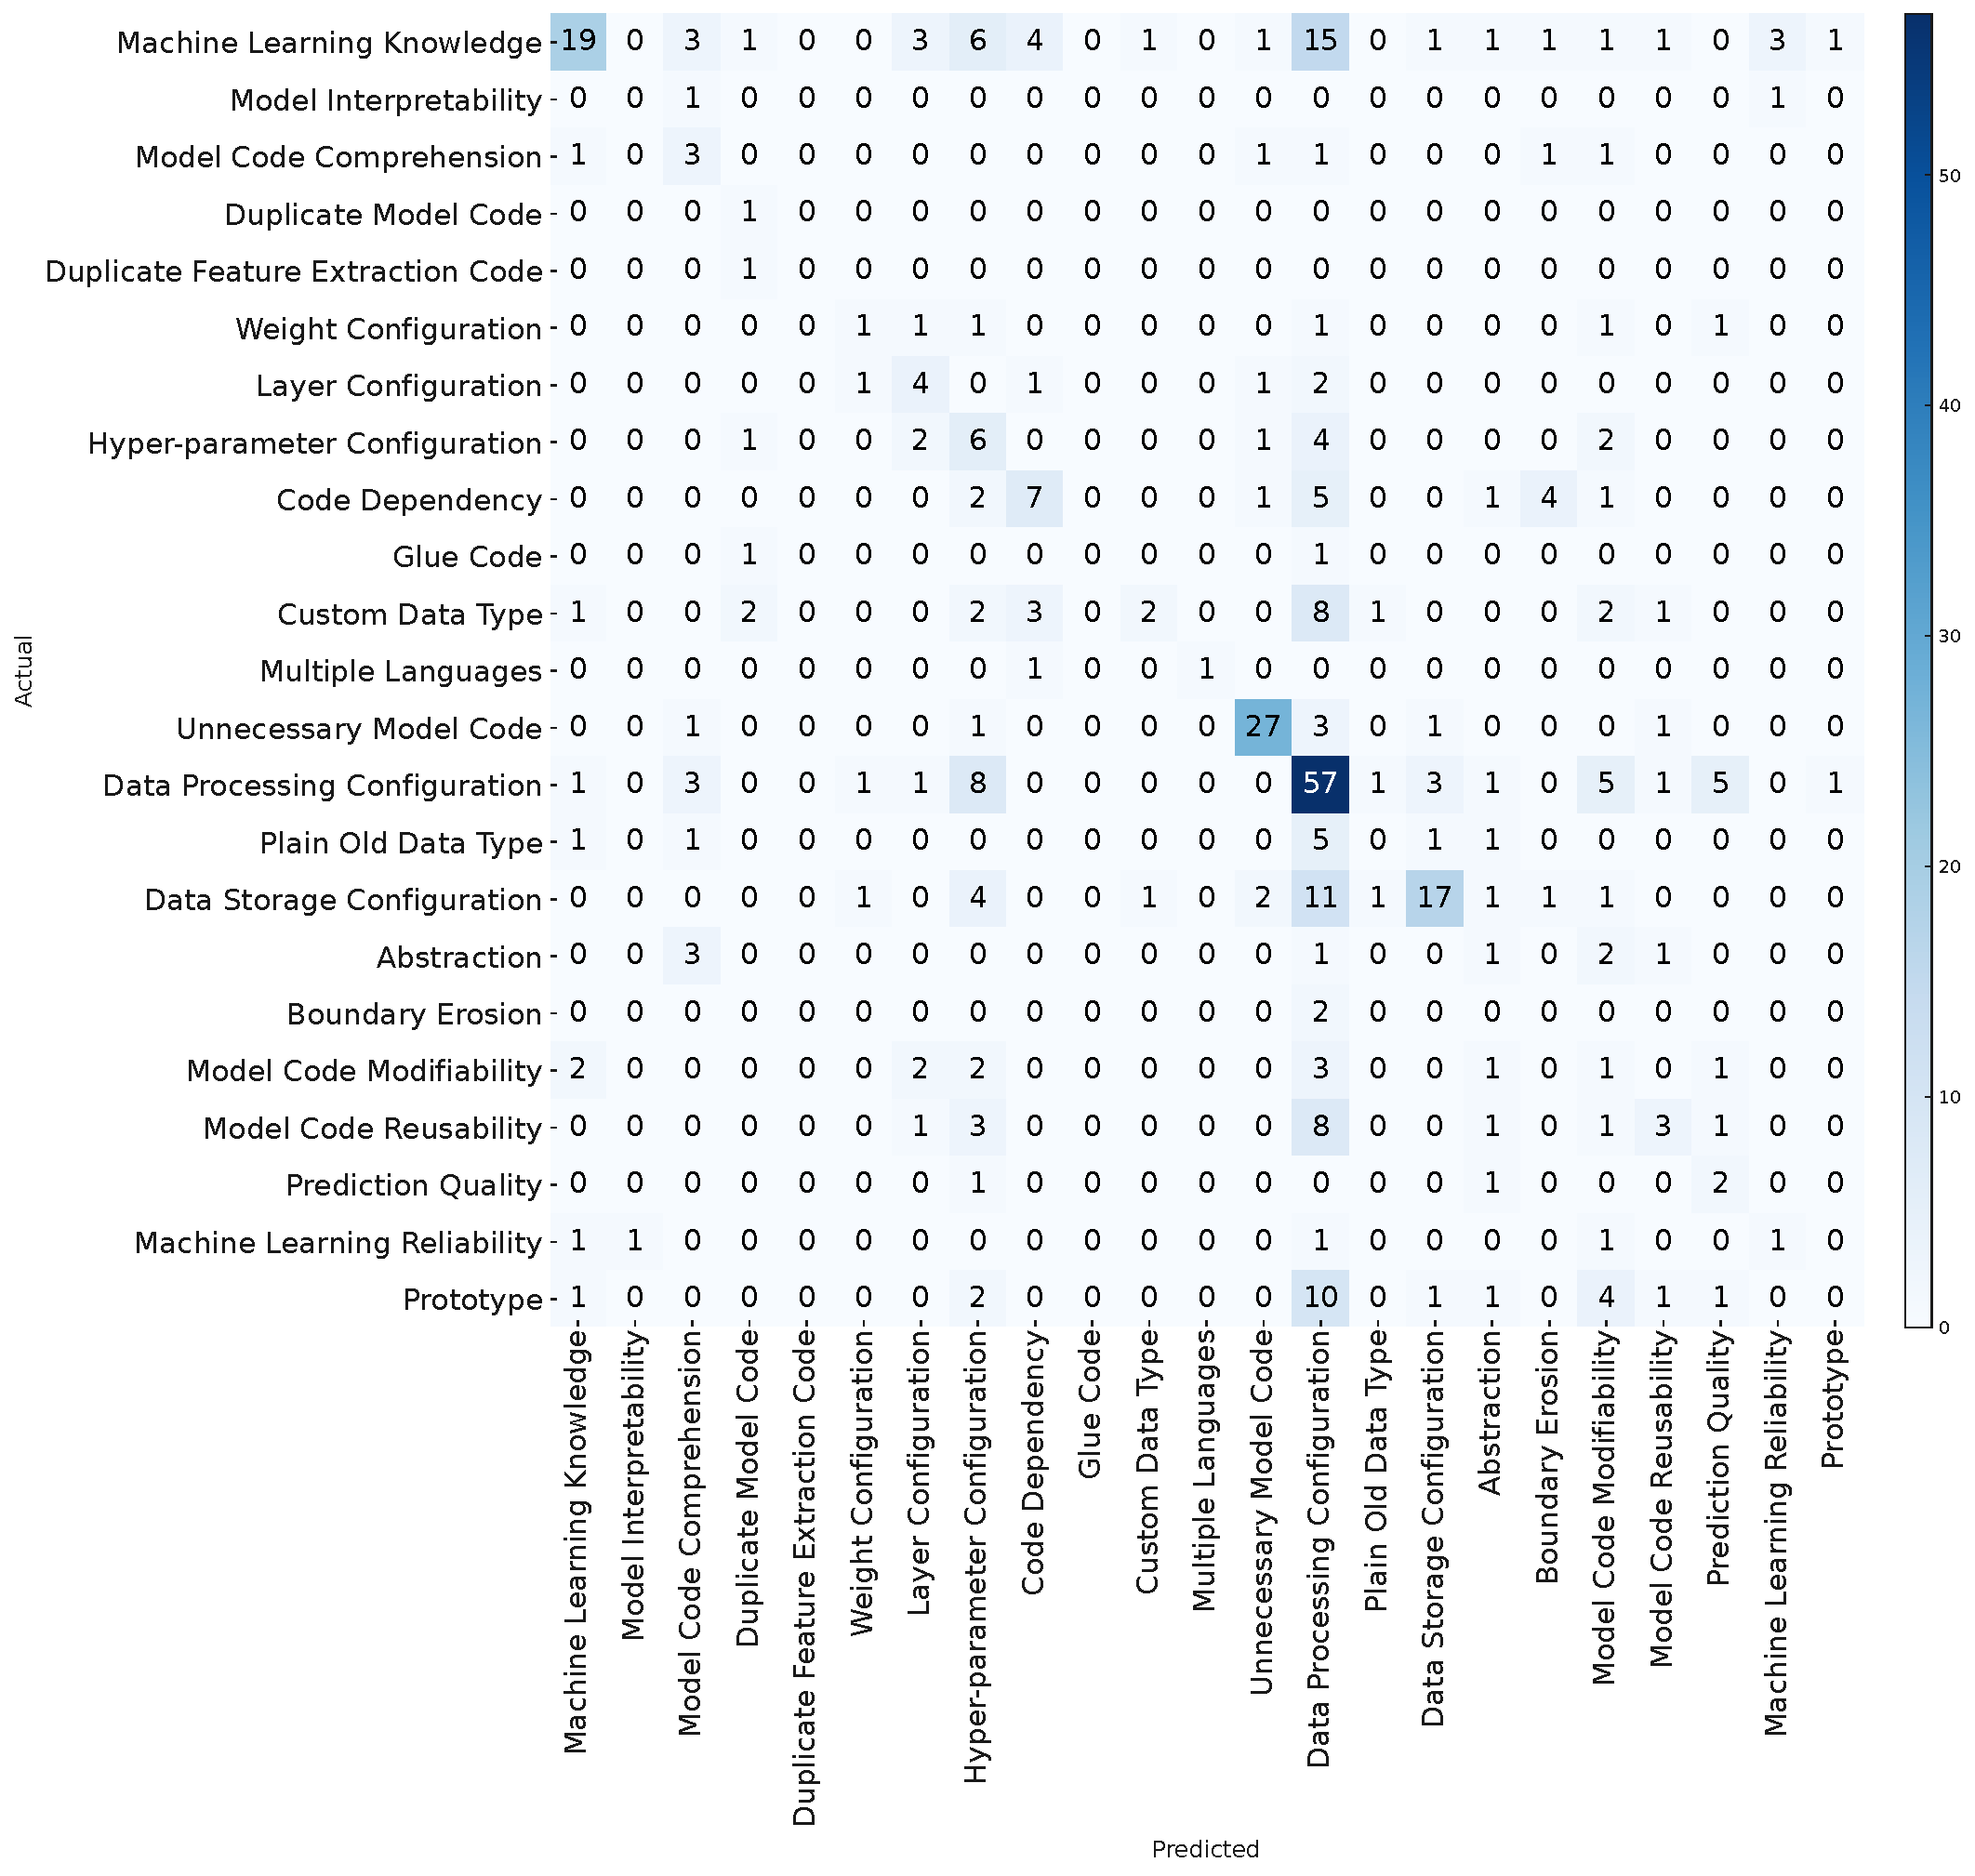
\includegraphics[width=0.7\textwidth]{confusion_matrix_heatmap_blues_v8_fix.pdf}
    \caption{Confusion Matrix for the best model.}
    \label{fig:confusion_matrix}
\end{figure}

We further analyze the confusion matrix of the best performing model, which is Qwen3-8B. As shown in the Figure \ref{fig:confusion_matrix}, the model performs relatively well on several high-frequency categories, especially Data Processing Configuration, Unnecessary Model Code, Machine Learning Knowledge, and Data Storage Configuration, which form the most visible diagonal blocks in the matrix. 

This pattern is consistent with the class distribution of the processed dataset, where these labels also have the largest supports. In particular, Data Processing Configuration shows the strongest diagonal count, indicating that the model can capture this category reasonably well under the best setting. At the same time, however, this label also acts as a major “attractor” class: many instances from Machine Learning Knowledge, Data Storage Configuration, Prototype, Custom Data Type, and Model Code Reusability are misclassified into it. This suggests that the model tends to over-predict broad data- and configuration-related debt when label boundaries are ambiguous. A similar confusion also appears among semantically adjacent configuration-related categories, such as Data Processing Configuration, Hyper-parameter Configuration, and Data Storage Configuration, indicating that although the model can recognize the general configuration nature of these comments, it still struggles to distinguish their finer-grained subtypes. In contrast, several minority or more abstract categories, such as Prototype, Plain Old Data Type, Model Interpretability, Glue Code, and Boundary Erosion, have very weak or even zero true positives, showing that current LLMs still have difficulty recognizing rare labels and categories with less explicit lexical cues. Overall, Figure \ref{fig:confusion_matrix} shows that the best model already captures the dominant structure of the label space, but its errors are concentrated on fine-grained distinctions among semantically overlapping ML-SATD types, which remains the main bottleneck for further performance improvement.

\begin{boxB}
\textbf{Findings:} (1) Combining different prompting strategies can further improve the performance of LLMs on fine-grained ML SATD classification.

(2) While not all selected model settings in the earlier RQs outperform the majority-class baseline, all combined configurations in Table~\ref{tab:combination_results} achieve clearly better results than both the random-guess and majority-class baselines.

(3) The best-performing configuration is Qwen3-8B under vanilla prompting with three examples and manually written Chain-of-Thought, achieving the highest weighted F1-score of \textbf{0.381}.
\end{boxB}










\section{Discussion}\label{sec:discussion}
In this section, we further summarize the practice guilderlines for using LLMs for fine-grained SATD classification and lessons learned from the experiments.

For the LLM selection, we suggest using the new reasoning models which can achieve better results than the traditional LLMs without reasoning. In our experiments, the Qwen3-series can achieve better results than the GPT-oss-20B series, although the later have more parameters. We recommend using Qwen3-series to do this task.

For the prompting methods, providing the detailed defination of the tasks and give the model generated examples, and incorpate with the manully written Chain-of-Thought can make the models achieves best performance.


Results on different categories do not follow the distribution of the datasets. Analysis from the best performing models on this task shows that LLMs' performance on the 

LLMs not always follow the prompts. During our experiments, we find some of the results 


\section{Discussion}\label{sec:discussion}

Our results suggest that new reasoning LLMs are more suitable for fine-grained ML SATD classification than traditional non-reasoning models. In particular, the Qwen3 series consistently shows strong performance, and the best overall result is achieved by Qwen3-8B under vanilla prompting with three examples and manually written chain-of-thought. This indicates that, for this task, instruction-following and reasoning ability are more important than parameter size alone. In addition, code-oriented models do not consistently outperform general-purpose models, suggesting that the task requires not only code understanding but also the interpretation of maintenance intent and subtle semantic differences among labels.

Prompt design also plays a critical role. Vanilla and binary prompting consistently outperform hierarchical prompting, indicating that multi-stage decomposition introduces additional error propagation. Adding LLM-generated examples is generally beneficial, but more examples do not necessarily yield better results; in most cases, fewer than three examples are sufficient. Manually written chain-of-thought further improves performance, likely because it helps the model distinguish semantically overlapping labels more effectively. Therefore, an effective prompt for this task should include clear label definitions, a small number of representative examples, and lightweight reasoning guidance.

Finally, the category-level results show that classification difficulty does not simply follow label frequency. Although several high-frequency categories are recognized relatively well, the confusion matrix reveals that many errors are concentrated among semantically similar labels, especially data-, configuration-, and dependency-related types. More abstract or low-frequency categories remain difficult to classify reliably. Moreover, LLMs do not always strictly follow the required output format, which becomes more problematic in a 23-class fine-grained setting. Overall, while open LLMs already provide a promising training-free solution for this task, semantic overlap among labels and imperfect prompt following remain important challenges for future work.


\section{Threats to validity}\label{sec:threats}
In this section, we will describe the threats that can affect the validity of our study.

\paragraph{Internal validity}

We test our results on a famous and widely used dataset due to the limited dataset available in this area. Some concerns about the generalized may rised about the results on the other datasets. We think the LLMs have a strong ability to performance well on other datasets, and these results found in our paper can generalized to other datasets and other models as well.

\paragraph{External validity} 
During our testing, we selected the open sourced LLMs due to the reasons of private. Some private code in the company are not suitable for senting to the online LLMs and these open sourced LLMs are the best option for develop in their own service and doing this task. Our results best show the performance of these models. The evouluation of these LLMs are very repaid and some new LLMs are emeraged after we finished the experiments. Further work can include these new models.

\section{Conclusion}\label{sec:conclusion}

This paper presents the first large-scale empirical study on the effectiveness of open LLMs for fine-grained ML-SATD classification. Using the O'Brien dataset with 23 ML-specialized SATD types, we evaluated nine representative open LLMs and systematically studied the impact of prompting strategies, LLM-generated examples, reasoning mode, and their combinations. Our results show that prompt design is critical for this task: vanilla and binary prompting consistently outperform hierarchical prompting, a small number of examples is generally more effective than using many examples, and reasoning further improves performance. Among all evaluated settings, the best result is achieved by Qwen3-8B with vanilla prompting, three generated examples, and manually written chain-of-thought, reaching a weighted F1-score of 0.381.

Overall, our findings demonstrate that open LLMs provide a practical and training-free solution for fine-grained ML-SATD classification under data-scarce and highly imbalanced settings. Beyond establishing a strong baseline, this study also offers concrete guidance for model selection and prompt design in this task. At the same time, the results suggest that fine-grained ML-SATD classification remains challenging, especially because of the sparsity of many labels and the semantic overlap among debt types. Future work can extend this study by evaluating stronger closed-source and newly released models, validating the findings on additional ML-SATD datasets, and exploring more realistic settings such as multi-label classification and broader ML-specific technical debt management tasks.



%%
%% The acknowledgments section is defined using the "acks" environment
%% (and NOT an unnumbered section). This ensures the proper
%% identification of the section in the article metadata, and the
%% consistent spelling of the heading.
% \begin{acks}
% To Robert, for the bagels and explaining CMYK and color spaces.
% \end{acks}

%%
%% The next two lines define the bibliography style to be used, and
%% the bibliography file.
\bibliographystyle{ACM-Reference-Format}
\bibliography{sample-base}


%%
%% If your work has an appendix, this is the place to put it.
\appendix

% \section{Appendix}

% \subsection{Part One}
% Different Prompting methods of ML SATD.


% \begin{table*}[ht]
\centering
\scriptsize
\caption{Definitions and Examples of the 23 Identified ML SATD Types: Awareness (AWR), Readability (RDB), Duplicate Code Elimination (DCE), Configurable Options (CFO), Code Dependency (CDD), Data Dependency (DTD), Modularity (MDL), Performance (PRF), and Scalability (SCL).}
\label{tab:ml_satd_types}
\begin{tabular}{
    >{\centering\arraybackslash}p{0.5cm}  % Dim. Name：短文本，居中
    >{\centering\arraybackslash}p{2cm}   % Type：稍长，居中
    p{7cm}                              % Definition：最长，左对齐，给足宽度
    p{2.8cm}                            % Example：较短，左对齐
}
\hline
\textbf{Dim. Name} & \textbf{Type} & \textbf{Definition} & \textbf{Example} \\
\hline
\multirow{2}{*}{AWR} & Machine Learning Knowledge & Machine learning software carries plenty of unique challenges. Uneducated solutions by unaware developers may have to be revisited. Machine learning models are a black box, causing poor understanding of model's functionality. This can lead to unknown behavior. & FIXME: can I backprop error through both TODO: Model Precision \\
\cline{2-4}
 & Model Interpretability & Machine learning models are a black box, causing poor understanding
of model’s functionality. This can lead to unknown behavior. & TODO: Model Precision \\
\hline
RDB & Model Code Comprehension & Model code carries extra legibility concerns that do not occur in traditional software. (i.e., poorly named temporary matrix variables). & TODO refactor second part of if statement when implementing live model prediction \\
\hline
\multirow{2}{*}{DCE} & Duplicate Model Code & Code duplication frequently occurs in model code. & TODO: Basically identical to 'test\_intra\_cv\_target\_transform' except for repeated KFold \\
\cline{2-4}
 & Duplicate Feature Extraction Code & Code duplication frequently occurs in feature extraction code. & XXX de-duplicate this with code from Montage somewhere? \\
\hline
\multirow{3}{*}{CFO} & Weight Configuration & Editing code that involves the weights of a ML model, or configuring a ML model's weights directly. & FIXME non-uniform sample weights not yet supported \\
\cline{2-4}
 & Layer Configuration & Editing code that deals with ML models' layers, or configuring a ML model's layers itself. & TODO: experiment with more layers \\
\cline{2-4}
 & Hyper-parameter Configuration & Configuring hyper-parameters of ML model, or editing the default values of off-the-shelf model. & TODO convert this to x/y params? \\
\hline
\multirow{5}{*}{CDD} & Machine Learning Dependency & When a needed change in ML software occurs because of its dependency on an external library or other piece of the ML software system. Usually indicates a condition that is waiting to be met before removal. & TODO add test for keypoints once their handling was improved in Convolve \\
\cline{2-4}
 & Glue Code & Supporting code written to interface with other code, inhibiting improvements due to peculiarities of dependent code. & FIXME XXX: Implement by rewriting functions above copied from autoresolve.py \\
 \cline{2-4}
 & Custom Data Type & Using data types provided by general-purpose packages can cause extensive inter-operating with external libraries. & TODO: Repeat\_elements and tf.split doesn't support dynamic splits. \\
 \cline{2-4}
 & Multiple Languages & Components written in other languages may introduce difficulties in ML development. & TODO(sonots): Implement in C++ \\
 \cline{2-4}
 & Unnecessary Model Code & Model code that either bottlenecks performance, is unreachable or deprecated, or is unnecessary and should be removed. & DEPRICATE? I don't think this is needed anymore \\
\hline
\multirow{3}{*}{DTD} & Data Processing Configuration & Configuring the way that data is processed either by editing the data directly, or by adding in new processing steps. & TODO: normalize true states \\
 \cline{2-4}
 & Plain Old Data Type & Using raw data types in ML causes confusion when interpreting processes. & TODO: handle record value which are lists; at least error \\
  \cline{2-4}
 & Data Storage Configuration & Configuring how data is represented within the source code (data structure) or how data is stored externally (database). & TODO json? \\
\hline
\multirow{4}{*}{MDL} & Abstraction & Lack of abstractions in ML systems and subsystems cause cascading changes when changes are introduced to one component. & TODO Split into separate functions \\
 \cline{2-4}
 & Boundary Erosion & Lack of boundaries between subsystems, creating difficulties when maintaining software and isolating changes made in ML software. & @todo nrows is for testing only! \\
  \cline{2-4}
 & Model Code Modifiability & Model code should be implemented in ways that enable easy maintenance and future modifications. & TODO init this somewhere else in a more principled way \\
  \cline{2-4}
 & Model Code Reusability & Model code should be generalized to be able to be reused in varying situations. & TODO: At the moment LHUC is RNN specific. \\
\hline
\multirow{2}{*}{PRF} & Prediction Quality & Previous work in evaluating ML workflows shows that changes may affect performance. & TODO: compare the performance! \\
 \cline{2-4}
 & Machine Learning Reliability & Machine learning models' functionalities are determined by the quality of their data, measures should be in place to ensure robustness. & TODO: extract an eval func more robustly \\
\hline
SCL & Prototype & Small-scale prototypes being deployed into full systems can be dangerous. & TODO: This matching process is slow. Make it faster; avoid loops where possible. \\
\hline
\end{tabular}
\end{table*}
% \begin{table}[htbp]
  \centering
  \small
  \caption{Results of different models under Vanilla and Binary prompting settings}
  \label{tab:vanilla_binary_CoT}
  \setlength{\tabcolsep}{6pt}
  \renewcommand{\arraystretch}{1.15}
  \begin{tabular}{l*{6}{c}}
    \toprule
    \multirow{2}{*}{Model} &
      \multicolumn{3}{c}{Vanilla\_CoT} &
      \multicolumn{3}{c}{Binary\_CoT} \\
    \cmidrule(lr){2-4}\cmidrule(lr){5-7}
    & precision & recall & f1
    & precision & recall & f1 \\
    \midrule
    Qwen3-8B                  & 0.356 & 0.333 & 0.295 & 0.389 & 0.349 & 0.333 \\
    Qwen3-14B                 & \textbf{0.472} & \textbf{0.384} & \textbf{0.363} & 0.400 & 0.336 & 0.313 \\
    Qwen2.5-Coder-7B-Instruct & 0.351 & 0.310 & 0.289 & 0.407 & 0.316 & 0.300 \\
    gemma-2-9b                & 0.355 & 0.288 & 0.275 & 0.382 & 0.295 & 0.297 \\
    gemma-3-12b               & 0.390 & 0.285 & 0.270 & 0.381 & 0.290 & 0.292 \\
    codegemma-1.1-7b-it       & 0.394 & 0.239 & 0.218 & \textbf{0.450} & 0.244 & 0.231 \\
    Llama-3.1-8B-Instruct     & 0.213 & 0.178 & 0.141 & 0.321 & 0.155 & 0.155 \\
    CodeLlama-7b-Instruct-hf  & 0.161 & 0.102 & 0.071 & 0.135 & 0.066 & 0.065 \\
    gpt-oss-20b               & 0.427 & 0.359 & 0.345 & 0.447 & \textbf{0.372} & \textbf{0.362} \\
    \bottomrule
  \end{tabular}
\end{table}
% \begin{table*}[ht]
\centering
\small
\caption{Definition of the father categories}
\label{tab:Super_def}
\begin{tabularx}{\textwidth}{
    >{\centering\arraybackslash}p{0.8cm}
    >{\raggedright\arraybackslash}X 
    >{\raggedright\arraybackslash}X 
}
\hline
\textbf{Dim. Name} & \textbf{Definition} & \textbf{Example Symptoms} \\
\hline
\multirow{4}{*}{AWR} & Lack of developer understanding or certainty about ML algorithms, APIs, data, or model behavior. Often arises due to ``black box'' nature of ML models. & Doubts on correctness, API usage uncertainty, unclear design decisions, unknown error causes, lack of domain knowledge. \\
\hline
\multirow{3}{*}{RDB} & Model code has poor legibility or unclear logic, especially in ML contexts (e.g., poorly named variables, dense math code). & Refactoring for clarity, simplifying complex statements, improving naming. \\
\hline
\multirow{2}{*}{DCE} & Identical or near-identical ML model or preprocessing logic appears in multiple places. & Repeated feature extraction, repeated model evaluation loops. \\
\hline
\multirow{3}{*}{CFO} & Missing or poorly implemented configuration points for weights, network layers, or model parameters. & Hard-coded parameters, unimplemented config flags, missing flexibility for experiments. \\
\hline
\multirow{3}{*}{CDD} & Code depends on other code or libraries in a way that blocks maintenance, requires workarounds, or is outdated. & Waiting for library updates, integration hacks, dependency-induced bugs, deprecated model code. \\
\hline
\multirow{3}{*}{DTD} & Issues in how data is processed, represented, or stored that hinder maintainability or correctness. & Missing preprocessing steps, poor choice of data formats, unoptimized storage. \\
\hline
\multirow{3}{*}{MDL} & Poor modular boundaries or design make the system harder to evolve, reuse, or maintain. & Missing abstractions, test parameters used in production, model-specific code that should be generalized. \\
\hline
\multirow{3}{*}{PRF} & Performance or robustness is insufficient, requiring evaluation, optimization, or reliability improvement. & Model accuracy concerns, robustness checks, performance comparisons. \\
\hline
\multirow{2}{*}{SCL} & Prototype-level code is used in production without scaling optimizations. & Inefficient loops, naive algorithms, lack of batching/parallelism. \\
\hline
\end{tabularx}
\end{table*}
\begin{table}[htbp]
  \centering
  \caption{Results of layered hybrid setting}
  \label{tab:layered-hybrid}
  \setlength{\tabcolsep}{6pt}
  \renewcommand{\arraystretch}{1.15}
  \resizebox{\textwidth}{!}{%
  \begin{tabular}{l*{9}{c}}
    \toprule
    \multirow{2}{*}{Type} &
      \multicolumn{3}{c}{Qwen3-14B} &
      \multicolumn{3}{c}{gemma-2-9b} &
      \multicolumn{3}{c}{gpt-oss-20b} \\
    \cmidrule(lr){2-4}\cmidrule(lr){5-7}\cmidrule(lr){8-10}
    & precision & recall & f1
    & precision & recall & f1
    & precision & recall & f1 \\
    \midrule
    AWR & \textbf{0.643} & 0.422 & 0.509 & 0.338 & \textbf{0.797} & 0.474 & 0.529 & 0.578 & \textbf{0.552} \\
    RDB & 0.062 & \textbf{0.625} & 0.112 & 0.103 & 0.375 & 0.162 & \textbf{0.167} & 0.500 & \textbf{0.250} \\
    DCE & 0.182 & \textbf{1.000} & 0.308 & \textbf{0.500} & \textbf{1.000} & \textbf{0.667} & 0.167 & \textbf{1.000} & 0.286 \\
    CFO & 0.187 & \textbf{0.452} & 0.264 & \textbf{0.245} & 0.387 & \textbf{0.300} & 0.184 & \textbf{0.452} & 0.262 \\
    CDD & 0.509 & \textbf{0.358} & \textbf{0.420} & 0.632 & 0.296 & 0.403 & \textbf{0.719} & 0.284 & 0.407 \\
    DTD & 0.718 & 0.204 & 0.318 & \textbf{0.773} & 0.248 & 0.376 & 0.656 & \textbf{0.431} & \textbf{0.520} \\
    MDL & 0.212 & \textbf{0.275} & 0.239 & 0.191 & 0.225 & 0.207 & \textbf{0.312} & 0.250 & \textbf{0.278} \\
    PRF & 0.250 & 0.333 & 0.286 & \textbf{0.385} & \textbf{0.556} & \textbf{0.455} & 0.060 & 0.333 & 0.102 \\
    SCL & 0.250 & \textbf{0.286} & \textbf{0.267} & 0.222 & 0.190 & 0.205 & \textbf{0.286} & 0.095 & 0.143 \\
    weighted avg & 0.517 & 0.318 & 0.350 & 0.519 & 0.366 & 0.364 & \textbf{0.530} & \textbf{0.392} & \textbf{0.420} \\
    \bottomrule
  \end{tabular}%
  }
\end{table}
\begin{table*}[ht]
\centering
\small
\caption{Definition of the father categories}
\label{tab:Super_def}
\setlength{\tabcolsep}{6pt}
\renewcommand{\arraystretch}{1.15}
\begin{tabularx}{\textwidth}{
    >{\raggedright\arraybackslash}p{3.4cm}
    >{\raggedright\arraybackslash}X
}
\hline
\textbf{Dim. Name} & \textbf{Definition} \\
\hline
Awareness (AWR) & Lack of developer understanding or certainty about ML algorithms, APIs, data, or model behavior. Often arises due to ``black box'' nature of ML models. \\
\hline
Readability (RDB) & Model code has poor legibility or unclear logic, especially in ML contexts (e.g., poorly named variables, dense math code). \\
\hline
Duplicate Code Elimination (DCE) & Identical or near-identical ML model or preprocessing logic appears in multiple places. \\
\hline
Configurable Options (CFO) & Missing or poorly implemented configuration points for weights, network layers, or model parameters. \\
\hline
Code Dependency (CDD) & Code depends on other code or libraries in a way that blocks maintenance, requires workarounds, or is outdated. \\
\hline
Data Dependency (DTD) & Issues in how data is processed, represented, or stored that hinder maintainability or correctness. \\
\hline
Modularity (MDL) & Poor modular boundaries or design make the system harder to evolve, reuse, or maintain. \\
\hline
Performance (PRF) & Performance or robustness is insufficient, requiring evaluation, optimization, or reliability improvement. \\
\hline
Scalability (SCL) & Prototype-level code is used in production without scaling optimizations. \\
\hline
\end{tabularx}
\end{table*}
% \begin{table}[h]
  \centering
  \small
  \caption{Results of the combination of different prompting strategies}
  \label{tab:combination_results}
  \setlength{\tabcolsep}{4pt}
  \renewcommand{\arraystretch}{1.15}
  \begin{tabular}{c c c c c c c c}
    \toprule
    \multirow{2}{*}{Setting} & \multirow{2}{*}{Metric} & \multicolumn{3}{c}{Vanilla prompting} & \multicolumn{3}{c}{Binary prompting} \\
    \cmidrule(lr){3-5}\cmidrule(lr){6-8}
    & & Qwen3-8B & Qwen3-14B & Gpt-oss-20B & Qwen3-8B & Qwen3-14B & Gpt-oss-20B \\
    \midrule

    \multirow{3}{*}{0} 
    & precision & 0.356 & \textbf{0.472} & 0.420 & 0.389 & 0.400 & 0.447 \\
    & recall    & 0.333 & \textbf{0.384} & 0.377 & 0.349 & 0.336 & \textbf{0.372} \\
    & f1        & 0.295 & 0.363 & 0.355 & 0.333 & 0.313 & 0.362 \\
    \midrule

    \multirow{3}{*}{1} 
    & precision & 0.397 & 0.433 & 0.405 & 0.412 & \textbf{0.447} & 0.430 \\
    & recall    & 0.359 & 0.364 & 0.359 & 0.354 & 0.359 & 0.356 \\
    & f1        & 0.345 & \textbf{0.365} & 0.349 & 0.358 & 0.363 & 0.355 \\
    \midrule

    \multirow{3}{*}{2} 
    & precision & 0.430 & 0.438 & \textbf{0.441} & 0.422 & 0.426 & 0.408 \\
    & recall    & 0.366 & 0.372 & 0.359 & 0.364 & 0.366 & 0.364 \\
    & f1        & 0.351 & 0.363 & 0.358 & 0.360 & 0.361 & 0.354 \\
    \midrule

    \multirow{3}{*}{3} 
    & precision & \textbf{0.445} & 0.425 & 0.436 & \textbf{0.424} & 0.435 & \textbf{0.450} \\
    & recall    & \textbf{0.389} & 0.361 & \textbf{0.382} & \textbf{0.382} & \textbf{0.382} & 0.369 \\
    & f1        & \textbf{0.381} & 0.360 & \textbf{0.375} & \textbf{0.377} & \textbf{0.377} & \textbf{0.371} \\
    \bottomrule
  \end{tabular}
\end{table}
% \begin{table}[htbp]
  \centering
  \small
  \caption{Thinking vs No-Thinking}
  \label{tab:model_prompt_thinking}
  \setlength{\tabcolsep}{4pt}
  \renewcommand{\arraystretch}{1.15}
  \begin{tabular}{c c c c c c}
    \toprule
    \multirow{2}{*}{Models} & \multirow{2}{*}{Metric} & \multicolumn{2}{c}{Vanilla} & \multicolumn{2}{c}{Binary} \\
    \cmidrule(lr){3-4}\cmidrule(lr){5-6}
    & & no-thinking & thinking & no-thinking & thinking \\
    \midrule
    \multirow{3}{*}{Qwen3-8B} & precision & 0.210 & \textbf{0.403} & 0.315 & 0.398 \\
    & recall & 0.196 & \textbf{0.326} & 0.237 & 0.267 \\
    & f1 & 0.168 & \textbf{0.303} & 0.249 & 0.282 \\
    \midrule
    \multirow{3}{*}{Qwen3-14B} & precision & 0.379 & 0.420 & 0.387 & \textbf{0.467} \\
    & recall & 0.305 & \textbf{0.366} & 0.280 & 0.308 \\
    & f1 & 0.302 & \textbf{0.341} & 0.284 & 0.300 \\
    \bottomrule
  \end{tabular}%
\end{table}
% % \usepackage{tabularx}

\begin{table}[ht!]
\centering
\small
\caption{Model-generated examples of the 23 Identified ML SATD Types.}
\label{tab:ml_satd_types}
\begin{tabularx}{\textwidth}{
    >{\centering\arraybackslash}p{0.8cm}
    >{\centering\arraybackslash}p{2.8cm}
    X 
}
\hline
\textbf{Dim. Name} & \textbf{Type} & \textbf{Example} \\
\hline
\multirow{4}{*}{AWR} & Machine Learning Knowledge & TODO: Confirm whether layer-norm before attention actually boosts convergence for small-batch training on this dataset \\
\cline{2-3}
 & Model Interpretability & TODO: Generate SHAP summary plot so users can see feature impact \\
\hline
\multirow{2}{*}{RDB} & Model Code Comprehension & TODO: break up monolithic function train\_eval\_predict() into clearer, single-purpose helpers \\
\hline
\multirow{4}{*}{DCE} & Duplicate Model Code & TODO: remove copy-pasted ConvBlock definition—reuse common\_layers.ConvBlock instead \\
\cline{2-3}
 & Duplicate Feature Extraction Code & XXX: text\_features\_v1 and text\_features\_v2 are copy-pasted—create one configurable pipeline \\
\hline
\multirow{6}{*}{CFO} & Weight Configuration & FIXME: pretrained checkpoint loads fp16 weights—add auto-cast to ensure dtype consistency \\
\cline{2-3}
 & Layer Configuration & TODO: swap BatchNorm for LayerNorm when depth $> 24$ \\ 
\cline{2-3}
 & Hyper-parameter Configuration & TODO: make learning\_rate schedule (cosine vs. linear) selectable via CLI flag \\
\hline
\multirow{10}{*}{CDD} & Machine Learning Dependency & TODO: bump scikit-learn to $\geq 1.6$ once conda forge wheels for arm64 become available \\  
\cline{2-3}
 & Glue Code & FIXME: adapter.py only exists to map old Predictor API to new one—rewrite consumers instead \\
\cline{2-3}
 & Custom Data Type & TODO: replace custom SparseTensorDict with standard torch.sparse\_coo\_tensor before exporting \\
\cline{2-3}
 & Multiple Languages & TODO: port custom attention kernel from CUDA C++ to Metal for macOS deployment \\
\cline{2-3}
 & Unnecessary Model Code & TODO: delete legacy compute\_grad\_stats(); superseded by torch.autograd.profiler \\
\hline
\multirow{6}{*}{DTD} & Data Processing Configuration & TODO: add configurable pipeline step to down-sample majority class before batching \\
\cline{2-3}
 & Plain Old Data Type & TODO: replace raw list of logits with a NamedTuple so callers know the order \\
\cline{2-3}
 & Data Storage Configuration & TODO: migrate checkpoint format from .pth to safetensors for safer serialization \\
\hline
\multirow{8}{*}{MDL} & Abstraction & TODO: extract common scoring logic into BaseMetric so each model wrapper isn’t re-implementing it \\
\cline{2-3}
 & Boundary Erosion & TODO: migrate training-time logging out of Trainer class; should live in metrics.logger \\
\cline{2-3}
 & Model Code Modifiability & TODO: move hyper-parameter defaults into config file so changing them doesn’t require code edits \\
\cline{2-3}
 & Model Code Reusability & TODO: abstract make\_encoder() so VisionTransformer and ResNet builders share the same backbone factory \\
\hline
\multirow{4}{*}{PRF} & Prediction Quality & TODO: rerun validation after enabling mixed-precision; confirm accuracy isn’t degraded \\
\cline{2-3}
 & Machine Learning Reliability & TODO: add sanity-check to reject examples with $> 20\%$ missing features before prediction \\
\hline
\multirow{2}{*}{SCL} & Prototype & TODO: replace the single-threaded demo server with a production-ready Gunicorn setup \\
\hline
\end{tabularx}
\end{table}
% \begin{table}[th!]
  \centering
  \caption{Few-shot result under the vanilla prompting setting}
  \label{tab:vanilla_few_shot}
  \setlength{\tabcolsep}{4pt}
  \renewcommand{\arraystretch}{1.15}
  
  \resizebox{\textwidth}{!}{%
  \begin{tabular}{
    >{\centering\arraybackslash}p{1cm}
    >{\centering\arraybackslash}p{1.2cm}
    *{10}{>{\centering\arraybackslash}p{1.9cm}}
  }
    \toprule
    & & Qwen3-8B & Qwen3-14B & Qwen2.5-Coder-7B-Instruct & gemma-2-9b & gemma-3-12b & codegemma-1.1-7b-it & Llama-3.1-8B-Instruct & CodeLlama-7b-Instruct-hf & gpt-oss-20b \\
    \midrule
    % --- 0-shot ---
    \multirow{3}{*}{0} & precision & 0.210 & 0.379 & 0.315 & 0.370 & 0.412 & \textbf{0.308} & 0.231 & \textbf{0.214} & \textbf{0.434} \\
    & recall & 0.196 & 0.305 & \textbf{0.262} & 0.290 & 0.285 & 0.198 & 0.221 & 0.148 & 0.344 \\
    & f1 & 0.168 & 0.302 & \textbf{0.242} & 0.268 & \textbf{0.289} & 0.167 & 0.156 & 0.108 & 0.340 \\
    \midrule
    % --- 1-shot ---
    \multirow{3}{*}{1} & precision & 0.246 & 0.388 & 0.294 & 0.337 & 0.407 & 0.256 & \textbf{0.298} & 0.186 & 0.397 \\
    & recall & 0.232 & 0.275 & 0.244 & \textbf{0.310} & \textbf{0.303} & 0.229 & 0.214 & 0.142 & 0.356 \\
    & f1 & 0.208 & 0.287 & 0.230 & 0.275 & 0.263 & 0.195 & 0.189 & \textbf{0.140} & 0.346 \\
    \midrule
    % --- 2-shot ---
    \multirow{3}{*}{2} & precision & 0.256 & 0.419 & 0.297 & \textbf{0.378} & 0.401 & 0.284 & 0.237 & 0.189 & 0.431 \\
    & recall & 0.249 & 0.313 & 0.229 & 0.303 & 0.295 & \textbf{0.265} & 0.206 & 0.183 & \textbf{0.379} \\
    & f1 & 0.238 & 0.328 & 0.213 & \textbf{0.298} & 0.260 & \textbf{0.220} & 0.191 & 0.123 & \textbf{0.369} \\
    \midrule
    % --- 3-shot ---
    \multirow{3}{*}{3} & precision & 0.255 & \textbf{0.422} & \textbf{0.345} & 0.359 & \textbf{0.435} & 0.243 & 0.270 & 0.126 & 0.415 \\
    & recall & 0.260 & \textbf{0.321} & 0.234 & 0.298 & 0.275 & 0.237 & \textbf{0.226} & 0.186 & 0.344 \\
    & f1 & 0.234 & \textbf{0.338} & 0.231 & 0.278 & 0.234 & 0.195 & \textbf{0.223} & 0.124 & 0.345 \\
    \midrule
    % --- 5-shot ---
    \multirow{3}{*}{5} & precision & \textbf{0.302} & 0.368 & 0.293 & 0.355 & 0.406 & 0.251 & 0.250 & 0.144 & 0.402 \\
    & recall & \textbf{0.280} & 0.272 & 0.209 & 0.277 & 0.282 & 0.201 & 0.196 & 0.168 & 0.344 \\
    & f1 & \textbf{0.256} & 0.287 & 0.210 & 0.268 & 0.247 & 0.184 & 0.189 & 0.107 & 0.348 \\
    \midrule
    % --- 10-shot ---
    \multirow{3}{*}{10} & precision & 0.254 & 0.370 & 0.298 & 0.298 & 0.205 & 0.252 & 0.270 & 0.050 & 0.427 \\
    & recall & 0.224 & 0.277 & 0.204 & 0.234 & 0.226 & 0.191 & 0.201 & \textbf{0.224} & 0.349 \\
    & f1 & 0.222 & 0.287 & 0.206 & 0.220 & 0.170 & 0.158 & 0.185 & 0.082 & 0.352 \\
    \bottomrule
  \end{tabular}%
  }
\end{table}
% \begin{table}[t!]
  \centering
  \caption{Few-shot result under the binary prompting setting}
  \label{tab:binary_few_shot}
  \setlength{\tabcolsep}{4pt}
  \renewcommand{\arraystretch}{1.15}
  
  \resizebox{\textwidth}{!}{%
  \begin{tabular}{
    >{\centering\arraybackslash}p{1cm}
    >{\centering\arraybackslash}p{1.2cm}
    *{10}{>{\centering\arraybackslash}p{1.9cm}}
  }
    \toprule
    & & Qwen3-8B & Qwen3-14B & Qwen2.5-Coder-7B-Instruct & gemma-2-9b & gemma-3-12b & codegemma-1.1-7b-it & Llama-3.1-8B-Instruct & CodeLlama-7b-Instruct-hf & gpt-oss-20b \\
    \midrule
    % --- 0-shot ---
    \multirow{3}{*}{0} & precision & 0.315 & 0.387 & \textbf{0.406} & 0.407 & \textbf{0.404} & 0.291 & 0.301 & 0.109 & 0.397 \\
    & recall & 0.237 & 0.280 & \textbf{0.323} & 0.293 & 0.328 & 0.183 & 0.153 & 0.048 & 0.354 \\
    & f1 & 0.249 & 0.284 & \textbf{0.311} & 0.279 & \textbf{0.326} & 0.171 & 0.146 & 0.052 & 0.351 \\
    \midrule
    % --- 1-shot ---
    \multirow{3}{*}{1} & precision & 0.316 & 0.399 & 0.333 & 0.404 & 0.404 & \textbf{0.379} & 0.276 & 0.138 & \textbf{0.412} \\
    & recall & 0.265 & 0.282 & 0.298 & \textbf{0.300} & \textbf{0.338} & \textbf{0.234} & \textbf{0.211} & 0.061 & \textbf{0.356} \\
    & f1 & 0.258 & 0.302 & 0.282 & \textbf{0.312} & 0.324 & \textbf{0.218} & 0.203 & 0.067 & \textbf{0.357} \\
    \midrule
    % --- 2-shot ---
    \multirow{3}{*}{2} & precision & \textbf{0.352} & \textbf{0.456} & 0.354 & 0.416 & 0.383 & 0.281 & 0.369 & 0.147 & 0.397 \\
    & recall & 0.267 & 0.316 & 0.321 & 0.298 & 0.326 & 0.219 & 0.209 & 0.079 & 0.351 \\
    & f1 & 0.281 & 0.335 & 0.298 & 0.309 & 0.305 & 0.190 & \textbf{0.226} & 0.075 & 0.348 \\
    \midrule
    % --- 3-shot ---
    \multirow{3}{*}{3} & precision & 0.333 & 0.449 & 0.347 & 0.416 & 0.363 & 0.232 & 0.374 & 0.270 & 0.395 \\
    & recall & \textbf{0.285} & 0.316 & 0.293 & 0.290 & 0.300 & 0.209 & 0.201 & 0.089 & 0.354 \\
    & f1 & \textbf{0.284} & 0.337 & 0.272 & 0.305 & 0.288 & 0.149 & 0.207 & 0.092 & 0.351 \\
    \midrule
    % --- 5-shot ---
    \multirow{3}{*}{5} & precision & 0.346 & 0.452 & 0.377 & \textbf{0.419} & 0.402 & 0.287 & 0.348 & \textbf{0.309} & 0.405 \\
    & recall & 0.262 & \textbf{0.318} & 0.288 & 0.277 & 0.308 & 0.224 & 0.181 & 0.097 & 0.344 \\
    & f1 & 0.267 & \textbf{0.342} & 0.286 & 0.289 & 0.309 & 0.175 & 0.184 & 0.084 & 0.341 \\
    \midrule
    % --- 10-shot ---
    \multirow{3}{*}{10} & precision & 0.340 & 0.429 & 0.264 & 0.312 & 0.397 & 0.261 & \textbf{0.379} & 0.123 & 0.381 \\
    & recall & 0.234 & 0.285 & 0.183 & 0.186 & 0.270 & 0.173 & 0.191 & \textbf{0.122} & 0.338 \\
    & f1 & 0.250 & 0.301 & 0.189 & 0.191 & 0.282 & 0.156 & 0.205 & \textbf{0.099} & 0.334 \\
    \bottomrule
  \end{tabular}%
  }
\end{table}
% \begin{table}[ht]
  \centering
  \caption{basic new CoT results}
  \label{tab:basic_new_CoT_results}
  \setlength{\tabcolsep}{4pt}
  \renewcommand{\arraystretch}{1.15}
  
  \resizebox{\textwidth}{!}{%
  \begin{tabular}{
    >{\centering\arraybackslash}p{1cm}
    >{\centering\arraybackslash}p{1.2cm}
    *{8}{>{\centering\arraybackslash}p{1.9cm}}
  }
    \toprule
    & & Qwen3-8B & Qwen3-14B & gemma-2-9b & gemma-3-12b & Llama-3.1-8B-Instruct & gpt-oss-20b \\
    \midrule
    % --- 0-shot ---
    \multirow{3}{*}{0} & precision & 0.356 & \textbf{0.472} & 0.355 & \textbf{0.390} & 0.213 & 0.420 \\
    & recall & 0.333 & \textbf{0.384} & 0.288 & 0.285 & 0.178 & 0.377 \\
    & f1 & 0.295 & 0.363 & 0.275 & 0.270 & 0.141 & 0.355 \\
    \midrule
    % --- 1-shot ---
    \multirow{3}{*}{1} & precision & 0.397 & 0.433 & 0.333 & 0.302 & \textbf{0.312} & 0.405 \\
    & recall & 0.359 & 0.364 & 0.321 & 0.295 & \textbf{0.224} & 0.359 \\
    & f1 & 0.345 & \textbf{0.365} & 0.292 & 0.263 & \textbf{0.219} & 0.349 \\
    \midrule
    % --- 2-shot ---
    \multirow{3}{*}{2} & precision & 0.430 & 0.438 & 0.357 & 0.323 & 0.257 & \textbf{0.441} \\
    & recall & 0.366 & 0.372 & 0.331 & \textbf{0.308} & 0.183 & 0.359 \\
    & f1 & 0.351 & 0.363 & 0.310 & 0.280 & 0.199 & 0.358 \\
    \midrule
    % --- 3-shot ---
    \multirow{3}{*}{3} & precision & \textbf{0.445} & 0.425 & \textbf{0.368} & 0.382 & 0.302 & 0.436 \\
    & recall & \textbf{0.389} & 0.361 & \textbf{0.333} & 0.303 & 0.198 & \textbf{0.382} \\
    & f1 & \textbf{0.381} & 0.360 & \textbf{0.320} & \textbf{0.282} & 0.207 & \textbf{0.375} \\
    \bottomrule
  \end{tabular}%
  }
\end{table}
% \begin{table}[htbp]
  \centering
  \caption{bisection CoT results}
  \label{tab:bisection_CoT_results}
  \setlength{\tabcolsep}{4pt}
  \renewcommand{\arraystretch}{1.15}
  
  \resizebox{\textwidth}{!}{%
  \begin{tabular}{
    >{\centering\arraybackslash}p{1cm}
    >{\centering\arraybackslash}p{1.2cm}
    *{8}{>{\centering\arraybackslash}p{1.9cm}}
  }
    \toprule
    & & Qwen3-8B & Qwen3-14B & gemma-2-9b & gemma-3-12b & Llama-3.1-8B-Instruct & gpt-oss-20b \\
    \midrule
    % --- 0-shot ---
    \multirow{3}{*}{0} & precision & 0.389 & 0.400 & 0.382 & \textbf{0.381} & \textbf{0.321} & 0.447 \\
    & recall & 0.349 & 0.336 & 0.295 & 0.290 & 0.155 & \textbf{0.372} \\
    & f1 & 0.333 & 0.313 & 0.297 & 0.292 & 0.155 & 0.362 \\
    \midrule
    % --- 1-shot ---
    \multirow{3}{*}{1} & precision & 0.412 & \textbf{0.447} & 0.410 & 0.371 & 0.283 & 0.430 \\
    & recall & 0.354 & 0.359 & \textbf{0.313} & \textbf{0.328} & 0.176 & 0.356 \\
    & f1 & 0.358 & 0.363 & \textbf{0.331} & \textbf{0.310} & 0.190 & 0.355 \\
    \midrule
    % --- 2-shot ---
    \multirow{3}{*}{2} & precision & 0.422 & 0.426 & 0.405 & 0.368 & 0.282 & 0.408 \\
    & recall & 0.364 & 0.366 & 0.303 & 0.326 & \textbf{0.181} & 0.364 \\
    & f1 & 0.360 & 0.361 & 0.314 & 0.309 & \textbf{0.202} & 0.354 \\
    \midrule
    % --- 3-shot ---
    \multirow{3}{*}{3} & precision & \textbf{0.424} & 0.435 & \textbf{0.425} & 0.349 & 0.247 & \textbf{0.450} \\
    & recall & \textbf{0.382} & \textbf{0.382} & 0.298 & 0.318 & 0.160 & 0.369 \\
    & f1 & \textbf{0.377} & \textbf{0.377} & 0.316 & 0.301 & 0.171 & \textbf{0.371} \\
    \bottomrule
  \end{tabular}%
  }
\end{table}
% \begin{table}[ht]
\centering
\caption{Statistics of the processed dataset}
\label{tab:stats}
\begin{tabular}{lc}
\hline
\textbf{type} & \textbf{number} \\
\hline
Data Conf & 88 \\
MLKnow & 62 \\
DS Conf & 40 \\
UMC & 34 \\
CDT & 22 \\
Proto & 21 \\
MLDepend & 21 \\
MCR & 18 \\
HP Conf & 16 \\
MCM & 12 \\
Layer Conf & 9 \\
PODT & 9 \\
MCC & 8 \\
Abs & 8 \\
Weight Conf & 6 \\
MLRelia & 5 \\
PQ & 4 \\
BE & 2 \\
GC & 2 \\
MLInter & 2 \\
ML & 2 \\
DMC & 1 \\
DFEC & 1 \\
\textbf{Total} & \textbf{402} \\
\hline
\end{tabular}
\end{table}





\end{document}




